%
%
% UCSD Doctoral Dissertation Template
% -----------------------------------
% https://github.com/ucsd-thesis/ucsd-thesis
%
%
% ----------------------------------------------------------------------
% WARNING: 
%
%   This template has not endorced by OGS or any other official entity.
%   The official formatting guide can be obtained from OGS.
%   It can be found on the web here:
%   http://grad.ucsd.edu/_files/academic-affairs/Dissertations_Theses_Formatting_Manual.pdf
%
%   No guaranty is made that this LaTeX class conforms to the official UCSD guidelines.
%   Make sure that you check the final document against the Formatting Manual.
%  
%   That being said, this class has been routinely used for successful 
%   publication of doctoral theses.  
%
%   The ucsd.cls class files are only valid for doctoral dissertations.
%
%
% ----------------------------------------------------------------------
% GETTING STARTED:
%
%   Lots of information can be found on the project wiki:
%   http://code.google.com/p/ucsd-thesis/wiki/GettingStarted
%
%
%   To make a pdf from this template use the command:
%     pdflatex template
%
%
%   To get started please read the comments in this template file 
%   and make changes as appropriate.
%
%   If you successfully submit a thesis with this package please let us
%   know.
%
%
% ----------------------------------------------------------------------
% KNOWN ISSUES:
%
%   Currently only the 12pt size conforms to the UCSD requirements.
%   The 10pt and 11pt options make the footnote fonts too small.
%
%
% ----------------------------------------------------------------------
% HELP/CONTACT:
%
%   If you need help try the ucsd-thesis google group:
%   http://groups.google.com/group/ucsd-thesis
%
%
% ----------------------------------------------------------------------
% BUGS:
%
%   Please report all bugs at:
%   https://github.com/ucsd-thesis/ucsd-thesis/issues
%
%
% ----------------------------------------------------------------------
% More control of the formatting of your thesis can be achieved through
% modifications of the included LaTeX class files:
%
%   * ucsd.cls    -- Class file
%   * uct10.clo   -- Configuration files for font sizes 10pt, 11pt, 12pt
%     uct11.clo                            
%     uct12.clo
%
% ----------------------------------------------------------------------



% Setup the documentclass 
% default options: 12pt, oneside, final
%
% fonts: 10pt, 11pt, 12pt -- are valid for UCSD dissertations.
% sides: oneside, twoside -- note that two-sided theses are not accepted 
%                            by OGS.
% mode: draft, final      -- draft mode switches to single spacing, 
%                            removes hyperlinks, and places a black box
%                            at every overfull hbox (check these before
%                            submission).
% chapterheads            -- Include this if you want your chapters to read:
%                              Chapter 1
%                              Title of Chapter
%
%                            instead of
%                              1 Title of Chapter
\documentclass[12pt,chapterheads]{ucsd}

%packages added by vineet
\usepackage{subfigure}
\usepackage{verbatim}
\usepackage{textcomp} % for \textquotesingle

% Include all packages you need here.  
% Some standard options are suggested below.
%
% See the project wiki for information on how to use 
% these packages. Other useful packages are also listed there.
%
%   http://code.google.com/p/ucsd-thesis/wiki/GettingStarted



%% AMS PACKAGES - Chances are you will want some or all 
%    of these if writing a dissertation that includes equations.
%  \usepackage{amsmath, amscd, amssymb, amsthm}

%% GRAPHICX - This is the standard package for 
%    including graphics for latex/pdflatex.
\usepackage{scrextend}
\usepackage{pslatex}
\usepackage{graphicx}

%% CAPTION
% This overrides some of the ugliness in ucsd.cls and
% allows the text to be double-spaced while letting figures,
% tables, and footnotes to be single-spaced--all OGS requirements.
% NOTE: Must appear after graphics and ams math
\makeatletter
\gdef\@ptsize{2}% 12pt documents
\let\@currsize\normalsize
\makeatother
\usepackage{setspace}
\doublespace
\usepackage[font=small, width=0.9\textwidth]{caption}

%% SUBFIG - Use this to place multiple images in a
%    single figure.  Subfig will handle placement and
%    proper captioning (e.g. Figure 1.2(a))
% \usepackage{subfig}

%% TIMES FONT - replacements for Computer Modern
%%   This package will replace the default font with a
%%   Times-Roman font with math support.
% \usepackage[T1]{fontenc}
% \usepackage{mathptmx}

%% INDEX
%   Uncomment the following two lines to create an index: 
% \usepackage{makeidx}
% \makeindex
%   You will need to uncomment the \printindex line near the
%   bibliography to display the index.  Use the command
% \index{keyword} 
%   within the text to create an entry in the index for keyword.
%   To compile a LaTeX document with an index the 'makeindex'
%   command will need to be run.  See the wiki for more details.

%% HYPERLINKS
%   To create a PDF with hyperlinks, you need to include the hyperref package.
%   THIS HAS TO BE THE LAST PACKAGE INCLUDED!
%   Note that the options plainpages=false and pdfpagelabels exist
%   to fix indexing associated with having both (ii) and (2) as pages.
%   Also, all links must be black according to OGS.
%   See: http://www.tex.ac.uk/cgi-bin/texfaq2html?label=hyperdupdest
%   Note: This may not work correctly with all DVI viewers (i.e. Yap breaks).
%   NOTE: hyperref will NOT work in draft mode, as noted above.
% \usepackage[colorlinks=true, pdfstartview=FitV, 
%             linkcolor=black, citecolor=black, 
%             urlcolor=black, plainpages=false,
%             pdfpagelabels]{hyperref}
% \hypersetup{ pdfauthor = {Your Name Here}, 
%              pdftitle = {The Title of The Dissertation}, 
%              pdfkeywords = {Keywords for Searching}, 
%              pdfcreator = {pdfLaTeX with hyperref package}, 
%              pdfproducer = {pdfLaTeX} }
% \urlstyle{same}
% \usepackage{bookmark}


%% CITATIONS
% Sets citation format
% and fixes up citations madness
\usepackage{microtype}  % avoids citations that hang into the margin


%% FOOTNOTE-MAGIC
% Enables footnotes in tables, re-referencing the same footnote multiple times.
\usepackage{footnote}
\makesavenoteenv{tabular}
\makesavenoteenv{table}


%% TABLE FORMATTING MADNESS
% Enable all sorts of fun table tricks
\usepackage{rotating}  % Enables the sideways environment (NCPW)
\usepackage{array}  % Enables "m" tabular environment http://ctan.org/pkg/array
\usepackage{booktabs}  % Enables \toprule  http://ctan.org/pkg/array



\begin{document}

%% FRONT MATTER
%
%  All of the front matter.
%  This includes the title, degree, dedication, vita, abstract, etc..
%  Modify the file template_frontmatter.tex to change these pages.
%
%
% UCSD Doctoral Dissertation Template
% -----------------------------------
% http://ucsd-thesis.googlecode.com
%
%


%% REQUIRED FIELDS -- Replace with the values appropriate to you

% No symbols, formulas, superscripts, or Greek letters are allowed
% in your title.
\title{Social Computing with Procedural Guidance for Complex Work}

\author{Vineet Pandey}
\degreeyear{2019}

% Master's Degree theses will NOT be formatted properly with this file.
\degreetitle{Doctor of Philosophy}

\field{Computer Science \& Engineering}
%\specialization{Human-Computer Interaction}  % If you have a specialization, add it here

\chair{Professor Scott R. Klemmer}
% Uncomment the next line iff you have a Co-Chair
% \cochair{Professor Cochair Semimaster}
%
% Or, uncomment the next line iff you have two equal Co-Chairs.
%\cochairs{Professor Chair Masterish}{Professor Chair Masterish}

%  The rest of the committee members  must be alphabetized by last name.
\othermembers{
Professor James D. Hollan\\
Professor Laurel Riek\\
Professor Robin Knight\\
Professor Donald Norman\\
}
\numberofmembers{5} % |chair| + |cochair| + |othermembers|


%% START THE FRONTMATTER
%
\begin{frontmatter}

%% TITLE PAGES
%
%  This command generates the title, copyright, and signature pages.
%

\makefrontmatter

%% DEDICATION
%
%  You have three choices here:
%    1. Use the ``dedication'' environment.
%       Put in the text you want, and everything will be formated for
%       you. You'll get a perfectly respectable dedication page.
%
%
%    2. Use the ``mydedication'' environment.  If you don't like the
%       formatting of option 1, use this environment and format things
%       however you wish.
%
%    3. If you don't want a dedication, it's not required.
%
%
\begin{dedication}
  To the adventure of life
\end{dedication}


% \begin{mydedication} % You are responsible for formatting here.
%   \vspace{1in}
%   \begin{flushleft}
% 	To me.
%   \end{flushleft}
%
%   \vspace{2in}
%   \begin{center}
% 	And you.
%   \end{center}
%
%   \vspace{2in}
%   \begin{flushright}
% 	Which equals us.
%   \end{flushright}
% \end{mydedication}



%% EPIGRAPH
%
%  The same choices that applied to the dedication apply here.
%
\begin{epigraph} % The style file will position the text for you.
  \emph{I don't do it for the 'Gram,\\
	 I do it for Compton}\\
  ---Kendrick Lamar
%, ELEMENT., {\it DAMN}
\end{epigraph}

% \begin{myepigraph} % You position the text yourself.
%   \vfil
%   \begin{center}
%     {\bf Think! It ain't illegal yet.}
%
% 	\emph{---George Clinton}
%   \end{center}
% \end{myepigraph}


%% SETUP THE TABLE OF CONTENTS
%
\tableofcontents
\listoffigures  % Comment if you don't have any figures
\listoftables   % Comment if you don't have any tables



%% ACKNOWLEDGEMENTS
%
%  While technically optional, you probably have someone to thank.
%  Also, a paragraph acknowledging all coauthors and publishers (if
%  you have any) is required in the acknowledgements page and as the
%  last paragraph of text at the end of each respective chapter. See
%  the OGS Formatting Manual for more information.
%
\begin{acknowledgements}

%from gut instinct
We thank all participants who used Gut Instinct and pro-vided feedback. We thank members of Design Lab, espe-cially Steven Dow and Derek Lomas, and Michael Bern-stein for their useful comments on this work. We thank Brian Soe and Aliff Macapinlac for help developing the Gut Instinct website and running pilot studies. A Google Re-search Award and gift from SAP helped support this work.

%from docent
We thank Docent participants for their feedback. We thank Chen Yang, Cody Doan, and Aliyah Clayton for help developing the website and running pilot studies. We thank Anupriya Tripathi and Nicolai Reeve for finding relevant scientific resources for the site, and Madeleine Ball for introducing Docent to the Open Humans community. A Google Research Award and gift from SAP helped support this work.

\end{acknowledgements}


%% VITA
%
%  A brief vita is required in a doctoral thesis. See the OGS
%  Formatting Manual for more information.
%
\begin{vitapage}
\begin{vita}
  \item[2011] B.~Engineering. in Computer Science \emph{cum laude}, Birla Institute of Technology \& Science, Pilani, India
  \item[2016] M.S.in Computer Science \& Engineering, University of California San Diego
  \item[2019] Ph.~D. in Computer Science \& Engineering, University of California San Diego
\end{vita}S
\begin{publications}
  \item Your Name, ``A Simple Proof Of The Riemann Hypothesis'', \emph{Annals of Math}, 314, 2007.
  \item Your Name, Euclid, ``There Are Lots Of Prime Numbers'', \emph{Journal of Primes}, 1, 300 B.C.
\end{publications}
\end{vitapage}


%% ABSTRACT
%
%  Doctoral dissertation abstracts should not exceed 350 words.
%   The abstract may continue to a second page if necessary.
%
\begin{abstract}
  This dissertation will be abstract.
\end{abstract}


\end{frontmatter}






%% DISSERTATION

% A common strategy here is to include files for each of the chapters. I.e.,
% Place the chapters is separate files: 
%   chapter1.tex, chapter2.tex
% Then use the commands:
%   %%%%%%%%%%%%%%%%%%%%%%%%%%%%%%%%%%%%%%%%%%%%%%%
%\chapter{Scaffolding Citizen-led Complex Knowledge Work}
\chapter{Social Computing for Complex Knowledge Work}

\begin{quote}
\emph{This dissertation explores how the following things happen. Complex work is hard. Needs learning. People do things in groups. Social computing misses learning (learning is around but not here). why your title is what it is, what that means, how you set up your arguments, and what claims your introductory chapter makes. Current online platforms (like Facebook) are built on insights from psychology about capturing people’s attention. My research instead takes a more socially responsible approach by integrating learning theory and collaboration for people to perform complex work such as generating and evaluating scientific theories. This has the potential to diversify the stakeholders and contributors to our future society.}
\end{quote}
\vspace{0.25in}

Social computing platforms have revolutionized how most people connect, communicate, and share. We increasingly connect with friends and strangers in different ways for a number of purposes. Friends and family can stay in constant touch with their loved ones. Strangers from different parts of the world discuss their ideas about their health. Increasingly, these connection opportunities have also translated to more active doing: people fund other's\'  ideas that traditional business places might balk at. Some have used social platforms to amplify their voice and bring about social changes. for instance, people in Sudan have taken down dictators [??]. By transforming how we communicate, share, and chat, social computing has become perhaps the greatest internet-fueled change of our times. 

%%interactive vis (social computing discussions) is awesome
% people can do stuff with hypotheses (test them?)
%    however, viz is hard (scientific work)
%        programming toolkits needed and impose burden (support needed to get started, reduce burden, and …)

However, the benefits of social computing are not distributed equally. While everyone has a voice, some have bigger loudspeakers than others: xx\% of most popular posts are from experts. While anyone can organize and bring changes, collective attempts to organize frequently fail. While anyone can learn from widely accessible research papers and articles, people create faulty insights from self-tracking and conspiracy theories abound. With this lens, social computing seems less transformative but rather a highly scaled up version of the offline reality of limited expertise people live in. 
% 1 to 1 link with the first para

%\subsection{Pivot to people - People can do great things but need help...}
%Well, what are people good at? What are they motivated to do? 

%People have complementary knowledge in comparison to experts and are uninfected by expert biases; these insights are drawn from lived experience, both individual and collective.

Specific to this dissertation: While social computing platforms have vastly succeeded at keeping people engaged and sharing, they barely support \textit {citizen-led enquiry}. People have strong personal motivations and contextual insights. People possess a remarkable ability to identify patterns and create theories from their experiences [??]. While most people have an amazing breadth and depth of ideas, they lack the expertise to implement these ideas. To create knowledge, they need mental scaffolds for organizing complex work, domain knowledge to compose and execute the steps, and ways to ask for help. Experts benefit from conceptual knowledge, professional training, pre-existing organizational structure for collaboration, and direct access to resources. Currently, citizens lack these resources. social computing platforms where people spend ridiculous times provide little support. 

%this is the current state --  this is the big challenge, why is it a challenge
%% however, scaling good teaching is hard - kulkarni
%     this peer thing can be helpful (evidence from small studies)
%        however, this is challenging — 2 causes
%        interfaces need to provide scaffolding 


\begin{figure}[b] 
  \centering
  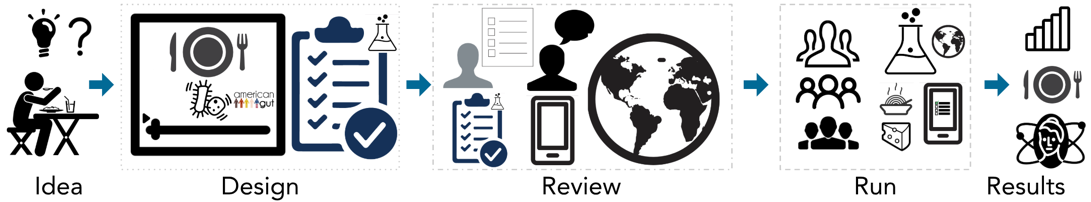
\includegraphics[width=1.0\textwidth]{figures/intro/intro-1}
  \caption[]
{The Gut Instinct platform enables anyone to transform their intuitions to hypotheses 
and then design and run experiments to test them [xx-xx]. Gut Instinct integrates 
conceptual learning embedded via short lectures and software-guided procedural 
learning to enable designing and reviewing experiments. Participants from around
 the world join experiments, follow instructions, and pro-vide data in response to 
automated data collection reminders. }
  \label{fig:intro-1}
\end{figure}

Consequently, this is unfortunate missed opportunity for both individuals and the world at large. Enabling peoplt to learn to perform personally meanignful work can help them answer their own questions. People's ideas can catalyze creating new knowledge that we are missing out on.  How might online systems support citizen-led knowledge work? 

Let''s reflect on this dual nature:  science can answer life-relevant questions but few know how to even get started. As a result, people fail to answer their questions and institutional science misses out on ideas from beyond the ivory tower. 

%one line to summarize my work -- see other intro

%two properties of classes help us - kulkarni
%this thesis leverages these two properties and provides a new class of benefits etc... 

%what helps us
%1. the scientific method is structured
%    1. even though creative and open-ended
%2. roles: people take them online
%    1. captures diversity — breadth
%    2. micro-expertise supports this explicitly 
%3. procedural learning: can teach people how to do things
%    1. captures learning — depth


This dissertation advances the design of social computing systems by integrating learning and collaboration to enable complex work such as generating and evaluating scientific theories. Over 600 people from 30 countries have self-organized to generate theories about the human microbiome and test them by running experiments. This dissertation raises the question: how can global communities create knowledge that meets their goals without waiting for experts to lead? 

Gut Instinct emodies this insight and introduces a collaborative citizen science platform for people to transform lived exes into scientific theories. 

%%%%%%%%%%%%%%%%%%%%%%%%%%%%%%
\section {People already do great things but struggle with complex tasks}

\subsection{People are awesome}
People design, build, and track to better understand and improve their health [?? dana lewis].  On numerous online fora, people share their intuitions, observations, folk theories, and even results from trying different approaches to improve their health, e.g. from simple ideas like ‘giving up drinking coffee to improve quality of sleep’ to tests and dietary approaches. People draw ideas from current research by reading and discussing papers. In many cases, these discussions are not just anecdotal but also derive from state-of-the-art scientific work. In some cases, people contribute back to scientific work as well.How can social computing platforms effectively enable people to do more personally meaningful work built upon their experiences and insights?

People’s curiosity, needs, and possibilities to do useful work is endless; however, traditional online systems don’t support them. Online fora encourage long, rambling discussions. Online learning provides conceptual lessons but people drop out and these are not linked to people’s needs.While learning resources like MOOCs abound, they hardly meet the need: many drop out, the lectures focus on conceptual knowledge, and lack the feedback needed to perform open-ended creative work. We know little about integrating learning resources and social computing affordances are far from each other. Moreover, currently both learning and work are not personal; can we change this? Lack of appropriate "learning abstractions" make complex work unrealistic.

The goal is to create environments for learning and collaboration through complex, personally meaningful work.

%%%%%%%%%%%%%%%%%%%%%%%%%%%%%%%%%%%%%%%%%%%%%%%%%%%
\subsection{Challenge: People' don't know what to do and how to do it}
Citizens have a different background than professional scientists; they have unique
 personal experiences but lack the years of domain training. Two major issues in 
enabling complex work on the internet are (diversity and scale?) 
quality of individual contribution and managing overall contributions from the crowd.
We desire social computing techniques that reliably enable a wide variety of people to 
contribute more than they naturally could and that manage the dependencies among
 a large set of tasks.

To create computational systems that leverage their strengths and mitigate the lack of training, this dissertation 
focuses on domains where the science is nascent, highly contextual, and personally motivating.
 Synthesizing the crowdsourcing literature and my experience highlights three challenges: 
poor signal-to-noise from crowds due to lack of training; inefficient collaboration without 
careful attention; and poor results (or no results at all) unless experts lead. 

To address  these concerns,  this dissertation introduces and evaluates peer production architectures 
and procedural learning.

\subsection{Scientific experimentation: An instance of complex knowledge work}
%here''s an example: experimentation 
Supporting complex knowledge work has been a challenge for Human Computer Interaction
 research (make specific). For instance, many people are interested in understanding and 
improving their health. Millions of peple from all over the world share their insights. 
Can't they run experiments for these?

Scientific experimentation features technical requirements and contextual choices 
that are inscrutable for a lay individual yet necessary for success [??]. While 
professional scientists and commercial ventures run experiments every day, with 
notable exceptions [??], empirical papers from non-professionals are 
vanishingly rare. This biases the questions asked, studies run, and knowledge 
created [??]. People have questions about their health, but lack the expertise 
and resources to scientifically investigate them. Broadening the pool of 
experimenters could help people investigate their curiosities, develop solutions 
to improve health and performance, and assist institutional researchers.


\textit{People lack the expertise to know what to do and how to do it.}. 
Success with complex creative activities requires procedural
knowledge (how to do things) in addition to conceptual
knowledge (facts). While many resources offer facts, procedural
learning is often ignored.The converse also holds, and much more often: novices are also
“uninfected” by all the knowledge that enables experts to
innovate.Sometimes, having a different background than experts can
be beneficial. Shared knowledge is great when it’s right, but
blocks progress when wrong. When false assumptions limit
experts, at least some novices are likely to be “uninfected”.
For example, GalaxyZoo volunteers discovered ‘green pea’
galaxies overlooked by scientists who mistakenly assumed
the green hue was merely an imaging artifact [54]. 


% kulkarni -- "This assessment requires bothcommon-sense knowledge to understand student work and the expertise to assess tacit criteria such as “well-designed” or “well-modularized” that cannot be completely articulated. Indeed, teaching such tacit criteria is an important goal in open-ended domains like design"


\textit{People lack a professional network to improve their work}. 
Furthermore,  how do people ask others for help? Who do they reach out to?

People are connected online and collectively have access to many resources.
In a large distributed community, there’s often someone who happens to 
have important relevant knowledge, usually drawing on a relevant but 
distant domain. Such distributed efforts are a type of lead-user innovation [31]. 
Having many people work on the same problem increases the odds that 
one will break through. Drawing on secondary expertise as inspiration can
 be an important agent of creativity because almost by definition, the 
combination is rare [10]. %Open \& crowd innovation builds up on contributions
 by diverse online participants, and a ‘bubbling up’ process for strong ideas [56].

While many hands make light work, novices need clear contribution opportunities. 
The crowdsourcing literature offers many good verification approaches for tasks 
with clear right or wrong answers – like whether two images represent the same 
product or what street number is written on a sign. However, verifying knowledge
 work necessitates a different approach because it requires making 
situationally-appropriate choices. 

%%%%%%%%%%%%%%%%%%%%%%%%%%%%%%%%%%%%%%%%%%%%%%%
\section{Thesis Statement and Contributions}
\noindent This dissertation investigates the question: how to enable people to perform personally meaningful work otherwise beyond their expertise? Underlying these investigations is the thesis:
%"My thesis statement is"
\begin{quote}
\emph{Providing task-specific guidance in social computing enables personally meaningful \& useful scientific work}
\end{quote}

This dissertation\textquotesingle s primary contribution is the idea of intergrating learning in social computing to enable groups of novices to perform complex, creative activities. The thesis achieves this integration by building a sequence of interactive prototypes that enable people to collaboratively generate and test hypotheses. In the process, the prototypes divide complex work into distinct activities: self-sourcing the design and crowdsourcing people''s inputs and data. Every prototype advances social computing further as a domain for deep, personally meaningful work. Beyond introducing learning abstractions, this dissertation carefully designs the affordances, support, and system to enable different users for different needs. 

 %To realize this idea, 
This dissertation makes three types of contributions: theoretical perspectives/techniques, real-world systems, and outcomes including empirical results, systems lessons, and dataset (Figure \ref{fig:contributions}). 

%%%%%%%%%
\subsection{Theoretical  Techniques}
Improving  work quality in social computing suggests deepening individual contributions and broadening participation by providing different contribution mechanisms.The former requires better learning tools and the latter requires better collaboration tools and dependency management. Consequently, this thesis' theoretical contributions include 1) principles to integrate guidance for complex tasks, and 2) ways to divide complex tasks into multiple roles or affordances.

%“..adapts and extends techniques from xxx” -  arvind

%system-led learning vs people-led
Traditional systems think of knowledge as being provided by the people, while we being the knowledge from the system itself.

%todo-introduce the learning and collaboraiton taxonomy here
\begin{figure}[b] 
  \centering
%  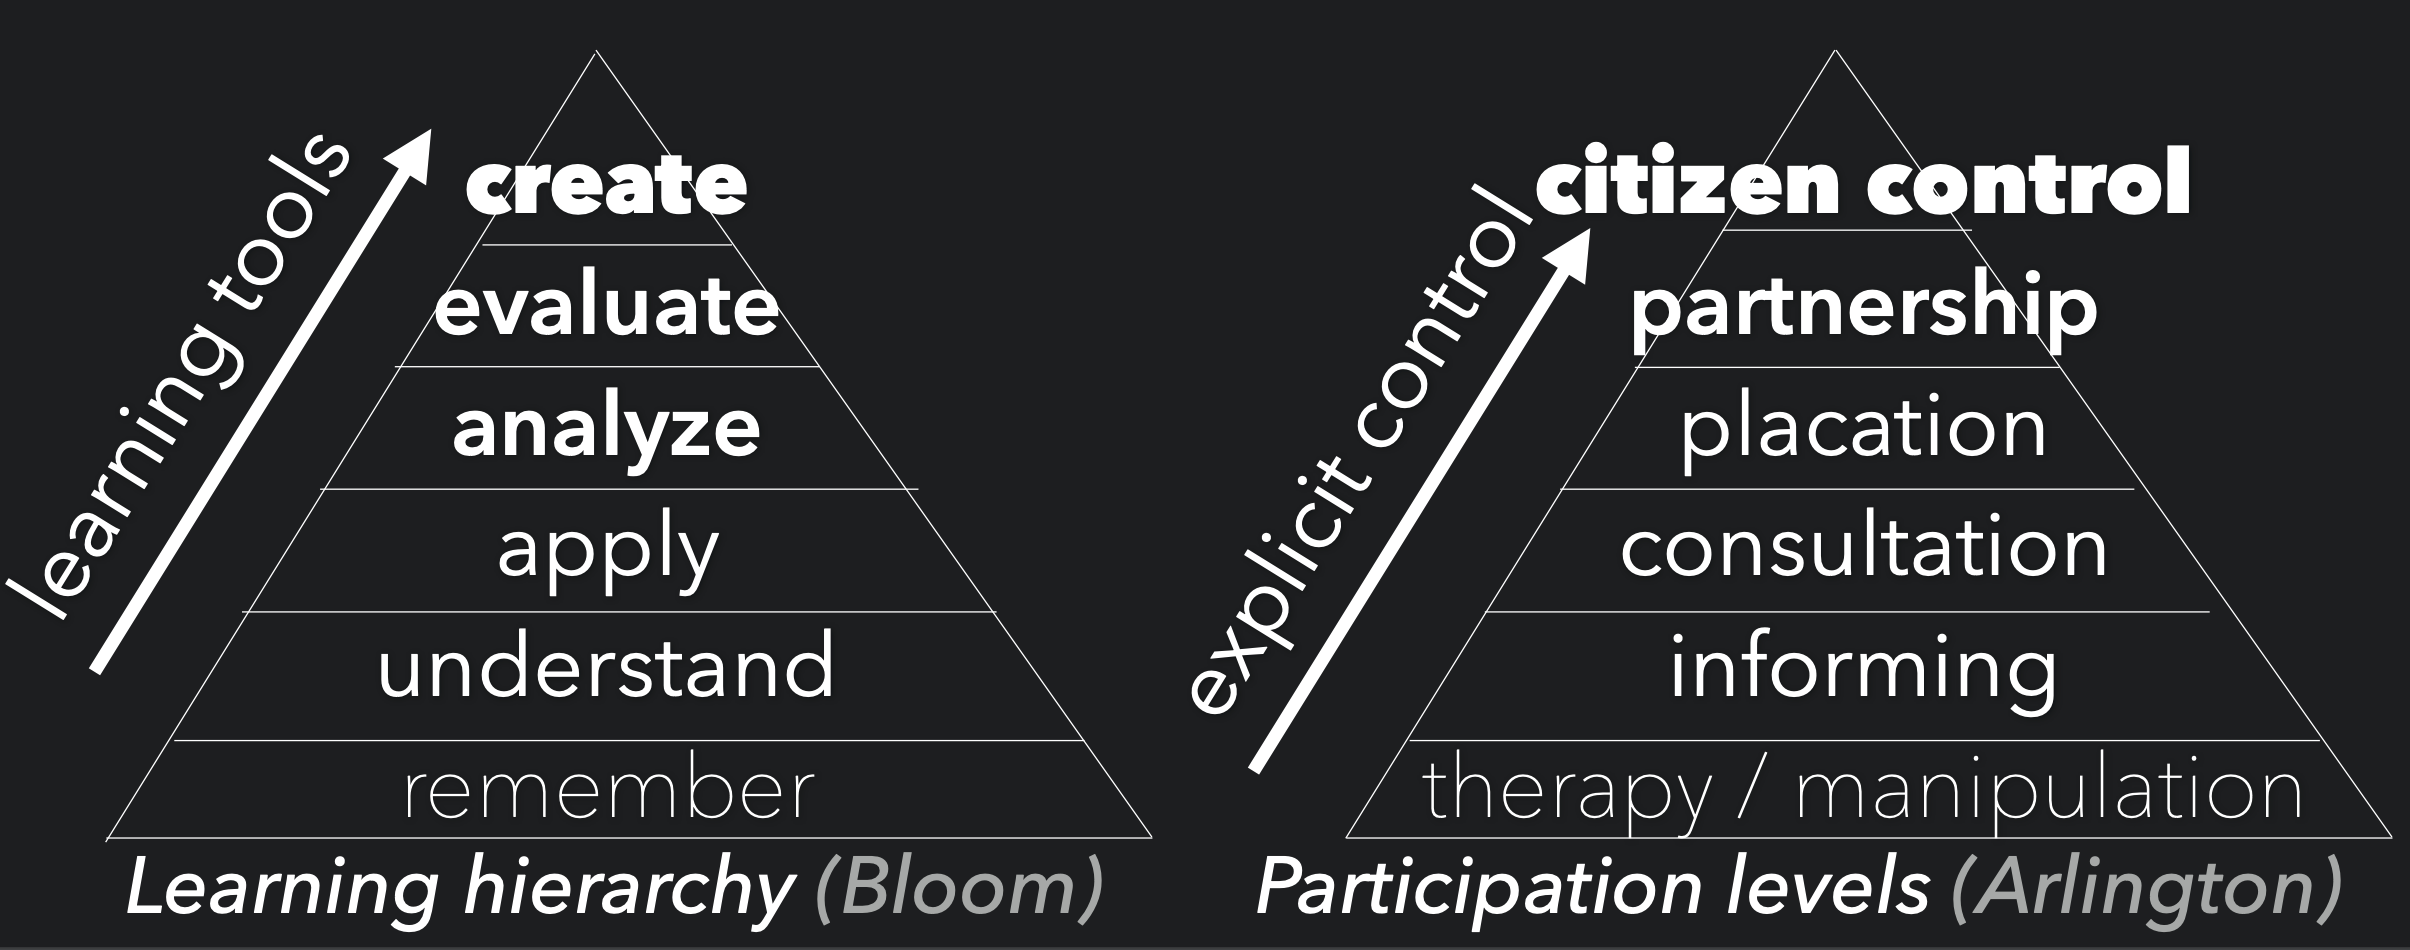
\includegraphics[width=1.0\textwidth]{figures/intro/intro-taxonomy}
  \caption[]
{Drawing from Maslow's hierarchy of learning and xx's hierarchy of contribution}
  \label{fig:intro-taxonomy}
\end{figure}

% come up with principles myself
%figure about conceptual and procedural learning 
\textit{Principles to integrate learning in social computing}: Learning broadly comprises conceptual (declarative) and procedural knowledge. Conceptual learning is where people learn what something is, learn about its features; this is a big part of current teaching. Typically, such learning is tested with test questions. In contrast, procedural learning teaches the {\it how} of things. How do you do x, y, or z.  Concpetual learning is useful when xxx while procedural learning is more useful when yyy.

To make useful contribution, people need to have a good working model of both the concepts and procedures for an activity. This dissertation enables this in two ways: 1) reifying conceptual bits in the software, and 2) providing procedural guidance with examples, checklists, and templates. Building on Maslow''s hierarchy~\ref{??}, it aims to push learning more up.

\textit{Principles to decompose Complex work to f(people, community, \& machines)}
% figure -- def needs one -- based on strengths and weaknesses
%fig - present a stack of things
The individual, groups of people, and machines possess complementary strengths. Individuals have personal motivation to do something; their lived experiences provide ideas that might be potentially novel. Groups of people might not be as motivated but might be willing to help by providing another set of eyes and complementary knowhow and insights from lived expeirences; they can help check biases with the diversity of their lived experiences. But since they are not as motivated, maybe limited affordances would be useful. Computers can implement things consistently to reduce biases but they cannot interpret open-ended instructions fairly in different contexts the way people can.  (todo- fix this to crisp english writing) (see slide deck)

Given these complementary strengths and limitations, this dissertation 1) begins every task with a heavy-handed implementation by an individual personally invested in that idea, 2) improves it with others'' feedback, and finally, 3) runs the idea with the help of automated software. For all these steps, the system manages the interdependencies beneath the sheets to reduce pressure on people. Building on xx's hierarchy~\ref{??}, it aims to push collaboration more up.

The efficacy of these techniques is borne out over multiple deployments. All these techniques have been put in systems as interfaces, intelligent backends, and so on... \\

%\begin{figure}[t!] 
%  \centering
%    \includegraphics[width=1.0\textwidth]{figures/img/intro/1-contributions}
%  \caption[Contributions of this dissertation]
%{Contributions of this dissertation including empirical results theoretical perspectives/techniques, real-world systems, and multiple outcomes}
%  \label{fig:contributions}
%\end{figure}

\subsection{User Interface and System Design}
%User interfaces and system design for efficient implementation
%figs needed to explicate 

While guidance techniques and role differentiation provide the building blocks, they are by themselves insufficient for useful higher-order collaborative work. These techniques need to be baked in simple, interactive interfaces. Multiple challenges show up for this question. First, the internet is a diverse community and have varying levels of expertise. So, the things need to be understandable to all. Second, people might have poor models of thiking about stuff and might frame their ideas and intuitions in weird ways.Third, the interface should make it easy to keep moving and get unstuck.  Too much information might make people struggle, so we need UIs for focused collaboration. 

This dissertation by bakes the techniques in the user interface  and by building a backend that is based on the principles of x, y, and z.

%System contributions
Gut Instinct  introduces a collaborative citizen science platform for people to transform lived exes into scientific theories. Gut Instinct frames the task of hypothesis-testing as a crowdsourcing problem, develops techniques and platform that supports different roles with just-in-time learning, and provides efficient backend support to automate simple tasks.

Gut Instinct divides multi-party collaboration into complementary tasks and supports them using different contribution mechanisms (like adding a question, editing a response) and roles (like experimenter, reviewer, participant). This provides people the flexibility to choose how much they’d like to contribute. Finally, Gut Instinct automatically manages multiple activities to reduce 
bias and experimenter/participant workload,such as randomized placement of 
people into conditions, maintaining anonymity, and collecting and cleaning data.


Take for instance, the state diagram — the edges represent what people need to do 
Roles Support via Just-in-time Skill Acquisition:  People take different roles--write up form galileo

%%"Furthermore, adding location information to photo collections is by itself insufficient for scenevisualization: we also need intuitive, interactive interfaces for exploring these scenes. There are several challenges faced in the design of such interfaces. First, unlike with Google Street View, where photos are taken at regular intervals, personal or Internet collections are typically an unstructured soup of photos. Nevertheless, the navigation controls should still be intuitive and exhibit regularity. Second, such controls should make it easy to find and explore the interesting parts of a scene, particularly for tourist sites."

%%%%%%%%%%%%%
\subsection{Outcomes}
\subsubsection{Empirical Results from Real-world Deployment}
expertise: limited; diversity: different countries; scale: some

\subsubsection{Dataset}
1. repo of hypotheses with rating
2. repo of experimental designs
3. ...

\subsubsection{Impact}
344 volunteers from 27 countries created 399 hypotheses about their health and the gut microbiome. Remarkably, microbiome scientists rated a fifth (75) of these hypotheses to have a scientifically valuable insight about a topic not covered by existing published work. Volunteers fleshed out 60 of these hypotheses into complete experimental designs. My entire work (code + data) is open source so others can edit, build, and experiment.

This dissertation has also enjoyed sufficient support in multiple research communities: Innovation researchers at MIT, online and offline fermentation and self-tracking communities, and citizen science groups. Finally, parts of the system have been taught in classrooms including CSCI 499: (Computing for Social Good) at USC. 

This work explores how online learning and process training systems, combined with
peer collaboration, can help people learn similar skills that
can be useful in scientific and design domains.


%%%%%%%%%%%%%%%%%%%%%%%%%%%%%%%%%%%%%%%%%%%
\section{Dissertation Roadmap}

%%%%%%%%%%%%%%%%%%%%%%%%%%%%%%%%%%%%%%%%%%%%%%%%%%%%%%%%%%%%%%%%%%
%todo- “we” refers to the set of authors…  -- see arvind

My dissertation demonstrates how we might draw on people’s diverse background knowledge, interest, and micro-expertise to expand scientific knowledge and push it in new directions. More specifically, the Gut Instinct platform that I have built instantiates these ideas enabling participants of the American Gut Project (the world’s largest crowdfunded citizen science project) to generate and experimentally investigate hypotheses (Figure 1). 

This dissertation creates the opportunity of harnessing humanity\textquotesingle s collective efforts to accomplish great goals.
s


"double quotes"


%The techniques make the idea concrete; the system operationalizes the techniques and makes them work; and the outcomes discuss the successes and failures of our approach.

%to people for them to perform personally meaningful work.
%My research prototypes collective systems for large-scale problems.
%Worldwide, people use online health fora to share insights and look for answers
%Iin short, to push people towards actively testing their ideas rather than just sharing them?  whether drinking kombucha really changes the gut constitution? In the absence of support and guidance, how can people do more? . 

%%1. novice-led
%    1. no experts
%    2. with other novices 
%2. personally meaningful 
%3. techniques
%    1. expert work to social computing 
%        1. ways to do that
%4. output
%    1. create new knowledge 

%   \chapter{Related Work}

\begin{quote}
\emph{This chapter summarizes research in citizen science, lead-user innovation, and social computing that inform the design of systems in this dissertation}. Citizen scientists have successfully solved expert-defined problems as sensors or algorithms. However, public involvement in scientific endeavors fail to provide a true participatory experience that is citizen-led and personally meaningful. Lead-user innovation provides a complementary setup. Lived experience, a tight feedback loop, and strong personal motivation enable people to create different and sometimes better products than experts; however, lead users rarely have access to training, conceptual knowledge, and pre-existing organizational structure for collaboration. Finally, social computing and crowdsourcing platforms support sharing potentially novel ideas but converting these to actionable plans requires expert guidance. This dissertation provides ways to integrate learning in social computing to enable deeper contributions from citizen scientists and lead users without expert involvement.
\end{quote}

%Professionals have the advantages of training, conceptual knowledge, and pre-existing organizational structure for collaboration and support; however, lead users rarely have access to such systematic support.

\begin{figure}[!h] 
  \centering
  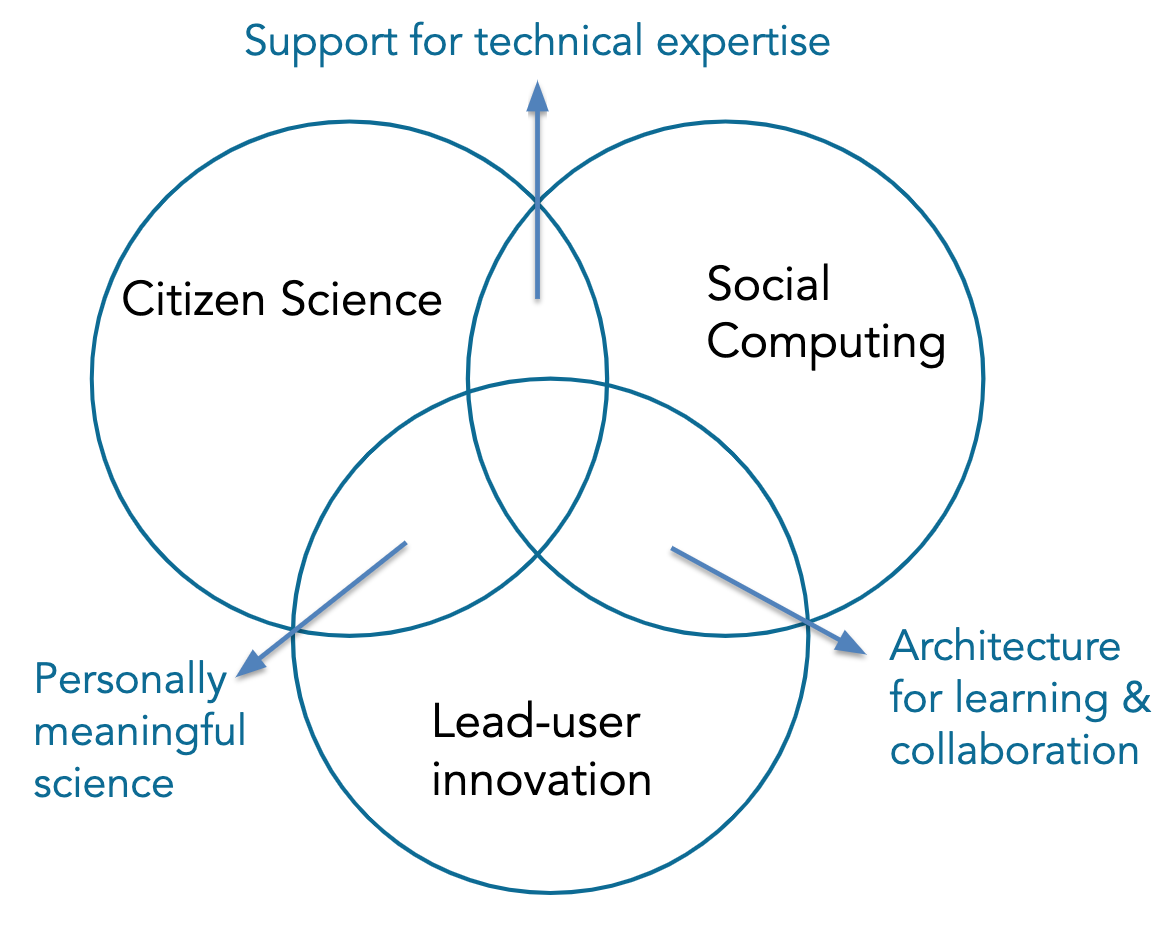
\includegraphics[width=0.6\textwidth]{figures/2-related/venn.png}
  \caption[]
{This dissertation draws from and contributes to citizen science, lead-user innovation, and social computing\index{related-1}}
  \label{fig:related-1}
\end{figure}

\vspace{0.25in}

%So, we find that there are three main challenges for citizen science: 1) make it personally meaningful, 2) deepen the contributions that citizens can make. 3. 1. Improve the quality of poor contributions — and improve the quality of max contributions     1. — hockey stick curve 
%%%%%%
\section{Science is increasingly networked but misses people’s lived experience }
Science is increasingly networked, multidisciplinary, and
open~\cite{Pandey2017}. For instance, \textit{LIGO}’s pathbreaking discovery of
gravitational waves brought together over 100 researchers
from over 100 institutions across 18 countries (ligo.org/about). 
Scientists increasingly share data and results faster (arxiv.org). 
Large scientific projects, like the \textit{Human Genome Project}, 
took to agile science by sharing methods, data, and insights to 
collaboratively speed discoveries. Scientists also form global 
collaborations to accelerate research in nascent scientific domains, 
like the Earth Microbiome project (earthmicrobiome.org).
At its best, institutional science has benefitted immensely
from large-scale global collaboration. Complementing this success,
many online projects enable people to help scientists~\cite{Nielsen2012}: annotating 
scientific papers~\cite{Good2013}; labeling galaxies~\cite{JordanRaddick2013}; and providing microbiome 
samples~\cite{McDonald2018}, CPU cycles (worldcommunitygrid.org), or personal data (openhumans.org). 
Efforts to further expand participation in scientific research are bearing fruit: \textit{Lab in the Wild} 
recruits anyone with an internet connection for behavioral studies~\cite{Reinecke2015}; and \textit{All of Us} aims 
to recruit one million Americans from all strata of society (allofus.nih.gov). Such collaborative efforts from experts 
and citizens suggest a new model for scientific work.

Often, when citizens participate in science, it is as \textit{embedded sensors} that 
are aggregated by experts. Public involvement in scientific endeavors continues
to be largely limited to performing tasks just beyond the reach of computers.
A classic example is \textit{Audubon}’s Christmas bird count, run since 1900
~\cite{Audubon2016}. Online examples include reporting flower blooms in
\textit{Project Budburst}~\cite{BoulderColorado2016}; recording wildlife activity~\cite{Faridani2009a};
identifying galaxies from satellite imagery in \textit{GalaxyZoo}~\cite{Zooniverse2007}; 
and biochemistry games: finding protein structures in \textit{Foldit}~\cite{Cooper2010}, 
synthesizing RNA molecules in \textit{EteRNA}~\cite{Lee2014}, and aligning 
nucleotide sequences in \textit{Phylo}~\cite{Kawrykow2012}. Distributed 
data contributions from people around the world—browsing online~\cite{Coviello2014}, using activity trackers, and joining scientific projects—have enabled valuable insights on topics including 
obesity~\cite{Althoff2017}, aesthetic preferences~\cite{Reinecke2014a}, sleep~\cite{F.lux2019}, and the human microbiome~\cite{McDonald2018a}. At their
best, these citizen science platforms yield novel insights.
For example, \textit{Foldit} players discovered protein structures
that helped scientists understand how the AIDS virus reproduces~\cite{Coren2011}. Why have such collaborative efforts succeeded?


%Different people provide different expertise that can vet claims and  fix mistakes~\cite{kane2009s}.
Collaboration benefits creativity when it brings different
 perspectives that build on each other; it impedes creativity (or worse, causes regression) 
when—through groupthink—it spreads biases rather than removing them~\cite{starbird2014rumors}. 
A humbling example of the power of fresh eyes: volunteer citizen scientists identified a new class of 
galaxies (\textit{green pea} galaxies) after researching green blots on \textit{Galaxy zoo} images; 
experts had dismissed these images as apparatus error~\cite{cardamone2009galaxy}.
This volunteer-led discovery demonstrates the need for fostering independent perspectives 
while simultaneously cultivating sufficient knowledge for meaningful domain contributions. 
Such collaboration requires strategic isolation: roviding just enough scaffolding to keep 
biases independent, while not stifling original ideas for bottom-up knowledge creation.

%This dissertation draws on the idea of people using  cognitive surplus to collaboratively answer scientific questions~\cite{Bonney2009}.


%%%% - where does this go
%Such bite-sized contributions is not without reason—a lot of
%scientific work requires deep conceptual knowledge and 
%training in scientific process to perform useful work. Most
%citizens lack the time, resources, and motivation to develop
%narrow, unique skillsets. Expanding the depth and breadth of work 
%performed by citizen science communities would be useful.

%\subsection{Citizen Scientists: From Collectors to Experimenters}
\subsection{Opportunity: Can people be scientists rather than just sensors?}
Citizens have successfully solved expert-defined problems as sensors or algorithms with a 
row-filling model of contribution.
In the quest to get people to track, measure, accumulate, or
sort both digital and analog data, citizen science has overlooked the massive 
opportunity of leveraging people’s unique advantages: our skills as reflective, 
creative thinkers who generate theories about the world, including ourselves.
People can offer more than just their data and perceptual
skills: they create theories, right or wrong, about a wide
range of topics including emotions~\cite{Johnson-Laird1992a}, motivation~\cite{Markus1991}, or
diet. These may be observational theories~\cite{Kempton1986}, folk theories
passed in a family/culture across generations~\cite{Gelman2011}, or ideas
brainstormed in online communities~\cite{23andme2016}. Perhaps, these intuitions 
can provide a starting point for independent, participatory experience that also assists the scientific community.

When are such personal experiences worth paying attention
to? For every intuition proven right, many more may be
closer to snake oil — e.g., the widespread belief in the utility
of probiotics despite limited evidence~\cite{Bonifait2009}. The global internet
increases the proliferation of both powerful and questionable
ideas: sharing speculation is fast while evaluation remains
slow. Moreover, people develop intuitions of cause and effect
that may or may not be correct. Current online forum
designs prioritize discussion — sharing personal details in
long, free-flowing text — over structure, succinctness, learning,
and potential scientific utility~\cite{Thomas2002}.

Advances in precision medicine have demonstrated the need
to engage people in uncovering and sharing insights~\cite{Aronson2015}. People
are highly motivated to improve their health outcomes,
more so if they suffer from a condition that severely affects
their quality of life, naturally forming communities. For example,
patients from the Amyotrophic Lateral Sclerosis
(ALS) community on \textit{Patients Like Me} (patientslikeme.com)
organized a study to track effects of Lithium on their symptoms
~\cite{Wicks2011}. This is not surprising; lead users excel at tackling
\textit{need-intensive} problems where they can use their lived
experiences to identify problems, try solutions, and readily
observe the effects~\cite{VonHippel2005}. Other organized communities like
\textit{Quantified Self} hope to uncover lifestyle patterns that may
improve their productivity and health outcomes. The word
‘self’ belies the fact that such movements are highly collaborative:
amateurs frequently share experiences and invite
feedback on online fora (patientslikeme.com) and blogs
(ibsgroup.org). Millions follow these ideas and some incorporate
these intuitions in their lives. What kinds of scaffolds
and structure may help people generate better ideas and implement them as actionable plans that
enable researchers to identify promising insights?

%How can people expand their insights into scientific work?

Most scientists develop their skills through an apprenticeship-
based graduate school experience. Apprenticeships emphasize
hands-on experience with individualized, taskspecific
feedback~\cite{schon1984reflective}. Scientists possess a wealth of declarative
knowledge about their domains (e.g., how to set up a
randomized controlled trial), and also procedural knowledge
—some narrow, some broad —towards getting things done
(e.g., improving fMRI signal intensity by having participants
consume cocoa beforehand~\cite{Francis2006}). This dissertation explores how
online learning and process training systems, combined with
peer collaboration, can help people learn similar skills that
can be useful in scientific domains.
%So, we find that there are three main challenges for citizen science: 1) make it personally meaningful, 2) deepen the contributions that citizens can make. 3. 1. Improve the quality of poor contributions — and improve the quality of max contributions     1. — hockey stick curve 
%WOULDN'T IT BE GREAT TO HAVE PEOPLE DESIGN AND RUN EXPERIMENTS AS AN INSTANCE OF COMPLEX SCIENTIFIC WORK
%Link to lead users -- people already doing personally meaningful work.. 

%%%%%%%%%%%%%%%%%%
\section{Lead users Succeed When They Know What to Do and How to Do It}
%“Lead users are rarely experts by themselves. They are novices who find themselves at the right place, with the right tools (that they might have created themselves), and who have the courage to follow through.” Lead users have created different—and in some cases better designs— than experts. 

%examples: UN example (see eric vh)

Lead-user innovation is both an inspiration and an application area for this dissertation. Lead users are
users of a product (or service) who experience advanced needs unmet by existing products~\cite{VonHippel2005}. The
power of lead-user innovation is that lived experience, a tight feedback loop, and strong personal
motivation can yield different and sometimes better products than experts [32]. For example, diabetes
patients have improved insulin delivery [47] and snowboarders have improved their binding
ergonomics. Lead users also collaborate online to build software
(github.com), create novel hardware \& reference designs
(openaps.org), and share personal data (quantifiedself.com,
openhumans.org). Some go further still, e.g., the transcranial
direct-current stimulation community draws ideas from scientific
papers to attempt self-experiments (reddit.com/r/tDCS). In a few exceptional cases, lead users have authored
scientific papers, e.g., Open Artificial Pancreas creator
Dana Lewis discussed the benefits and challenges of first-generation
automated insulin delivery at the 2016 American
Diabetes Conference~\cite{DanaLewis}.

Why do people do this? Curiosity, personal learning, and social
comparison are three reasons~\cite{Reinecke2015}. A massive interest in
personal genomics (over 1 million 23andme participants)
and the human microbiome (13,000 \textit{American
Gut} participants) demonstrates people’s yearning for self-understanding.
Users of these platforms send data, answer survey questions,
and discuss on fora. Some even use online lectures to understand
concepts of genes, phenotypes, and microbiota~\cite{23andMe2017, Knight2016}. 

\subsection{Opportunity: Providing lead users the expertise to tackle complex knowledge work}
Sometimes, having a different background
 than experts can be beneficial. Shared knowledge is great when it’s right, but blocks progress
 when wrong. When false assumptions limit experts, at least some novices are likely to be 
\textit{uninfected}. The converse also holds, and much more often: novices are also uninfected
by all the knowledge that enables experts to innovate. Lead users have an advantage when the key ingredient is experience intensive; experts retain the
advantage for \textit{solution-intensive} innovations [32]. In a large distributed community, 
there’s often someone who happens to have important relevant knowledge, usually 
drawing on a relevant but distant domain. Having many people work on the same problem 
increases the odds that one will break through. Drawing on secondary expertise as 
inspiration can be an important agent of creativity because almost by definition, the
 combination is rare~\cite{Boden2004}. 
%For example, GalaxyZoo volunteers discovered ‘green pea’ galaxies overlooked by scientists who mistakenly assumed the green hue was merely an imaging artifact~\cite{Tinati2015}. 

Community-driven approaches to understand personal
health and well-being largely reside outside the realm
of institutional science and medicine. While some fads and beliefs are 
questionable at best, on occasion communities
break new ground that may provide widespread value,
such as fecal transplants to alleviate \textit{Clostridium difficile} infection
symptoms~\cite{Brandt2012}. Some doctors recommend that patients
track their symptoms and reflect upon them to find
insights. Putting people in charge can help them find significant
relief for ailments like chronic migraine~\cite{Gawande2017} and provide
researchers and clinicians with useful patient data
(smartpatients.com). Insights from N\Hair=\Hair1 studies have helped
crack scientific puzzles about the working of the mind~\cite{V.S.Ramachandran1998},
heart, and microbes~\cite{Weisse2012}. 

Personal needs and challenges can be highly motivating but performing complex work still requires multiple rounds of trial and error. 
People need to know the genre of work and implement it correctly.  Professionals have the advantages of training, conceptual knowledge, 
pre-existing organizational structure for 
collaboration and support, and direct access to resources. Lead users either seek these resources from others or need to create them. 
Providing a correct and complete model for complex, structured activities might reduce efforts and improve the quality of results.
This dissertation reduces the gap between lead users' ideas and implementation by providing templates for 
genre work using just-in-time training and a collaboration platform to find others. This dissertation focuses on enabling people transform their idea to a controlled experiment as opposed to 
self-tracking or informal iteration which is the focus of most current citizen-led work in health.

\subsection {Case: Scientific experimentation is difficult}
While public contributions have supported institutional science; it’s rare for citizens to design
their own experiments. A number of health and behavioral research projects enlist citizens as helpers (e.g., \textit{HabitLab} [43]). 
\textit{CivilServant} enables online communities’ 
moderators to test policy ideas; moderators share these ideas with researchers who transform 
them to study designs [51]. Through the \textit{PatientsLikeMe} website (patientslikeme.com), citizens 
and scientists created a study investigating whether consuming lithium alleviated ALS symptoms [64]. 
While an initial scientific study had provided positive benefits, both this citizen science study and 
a subsequent university study did not find benefits. \textit{Tummy Trials} asked 
participants to generate health questions, introducing a protocol for self-experimentation 
combining ideation and self-tracking [36]. In all these cases, citizens rely on experts to provide sound experimental design.

Why is experimentation hard?  Despite a predetermined goal and a formalized process, experimentation
requires making situationally-appropriate decisions. A dependent variable may produce crisp
numbers but feedback on the experiment design itself is more multifarious. Good experiment
design is inherently user centered: how will participants interpret the instructions? Experiment
designers need awareness of others’ interpretation of their ideas and asks. Feedback and iteration
might be key to creative success, especially for novices. Providing feedback on experiment
designs requires knowing the success criteria and how to
help improve.  Feedback can be provided by experts~\cite{dow2012shepherding, schon1984reflective}, peers~\cite{Boud1995, Kulkarni2015b}, software~\cite{Dantoni2015, Head2017}, or even oneself~\cite{Boud1995,schon1984reflective}. While feedback from novices can
potentially improve both structure and content, it can also emphasize superficial issues over the
underlying structure~\cite{chi1981expertise}. Finally, successfully running an experiment
requires managing multiple processes such as random
assignment, anonymizing participant details, and sending
instructions and reminders for data collection.

%%%%%%%%%%%%%%%%%%%%%%%%%%%%%%%%%%%%%%%%%%%%%%%%%%%%%%%%%%%%%%%%%%%%
%But to understand that let's look at social computing ideas...

\section{Social Computing and Crowdsourcing Architectures for Complex Work}
Canonical crowdsourcing breaks larger tasks into microtasks; algorithms specify the division,
dependency, and agglomeration activities while workers perform small tasks supported by task-specific
guidelines~\cite{kittur2012future}. Leveraging existing expertise is one approach for complex knowledge work. One strategy
directly employs experts’ just-in-time feedback to improve crowd work~\cite{dow2012shepherding}. Workflows manage
experts for open-ended work like developing interactive prototypes~\cite{Retelny2014}. 
\textit{Flash Organizations} uses automated hiring, a hierarchy with a central leader, and optional 
team leaders for collaborative projects like product design~\cite{Valentine2017}.
Another strategy creates roles that enable more experienced crowd members to orchestrate
the work. \textit{Ensemble} supports leaders in guiding and constraining crowd 
contributions~\cite{Kim2014e}. Role-based approaches confer three benefits: 1) clean 
delineation of responsibilities improves chances of task completion, 2) clustering similar tasks 
reduces overhead and increases consistency; 3) people can decide their contribution levels. 
However, experts are expensive, in short supply, and sometimes prone to groupthink. 

Carefully-constructed interfaces can aid novices with task-specific expertise to solve problems 
that only experts previously could. \textit{Foldit} introduced 3D game for specifying low-energy protein 
structures via direct manipulation~\cite{Cooper2010}. Making a challenge visually salient is an 
effective way to on-board novices. For tasks that don’t have as a crisp visual analogue as protein
folding, people need better conceptual support. Prior work has explored collaborative hypothesis generation and testing on pre-existing data sets
~\cite{luther2009pathfinder,willett2011commentspace}. This dissertation offers a 
complementary contribution: enabling citizens to generate data on topics of personal interest.

One way to make complex tasks manageable is to divide them into distinct phases. 
Touchstone demonstrates the power of a semi-automated workflow integrating experiment 
design, testing, and analysis~\cite{Mackay2007}. Crowdsourcing has similarly innovated by 
creating distinct phases: break larger tasks into microtasks; algorithms specify the division, 
dependency, and agglomeration activities while workers perform small tasks supported by 
task-specific guidelines~\cite{lasecki2012real}. From these systems, our work draws the 
idea of dividing experimentation into multiple tasks—some self-sourced, others 
crowd-sourced; and introduce just-in-time domain expertise to perform these tasks. 

 
%How might groups of novices perform complex work like experimentation?
%Systems like Foldit and EteRNA powerfully show  how carefully-constructed interfaces provide
%novices with the task-specific expertise to solve problems that only experts previously 
%could~\cite{Cooper2010, Lasecki2012, Lee2014, Zooniverse2007}.

%%%%%%%
%%building up solution space - more work
\subsection{Learning resources at the right time}
Providing just-in-time supports, step-by-step instruction, and showing helpful supportive
 information are core ideas in instructional design~\cite{Kirschner2008}. Crowdsourcing 
systems leverage interactive guidance for specific tasks. For example, \textit{CrowdLayout} and 
\textit{Cicero} provide guidelines and static rules that workers use these to reason about their choices
 and improve network layouts~\cite{chen2019cicero, Singh:2018:CCD:3173574.3173806}. 
Others like \textit{CrowdSCIM} and \textit{Crowdclass} scaffold pre-task interventions~\cite{Lee2016,wang2018exploring}. 
While learning resources are distributed across the internet, they are rarely integrated with the task. 

Creative, open-ended work has rich pedagogical value. Online work, like 
online learning, requires appropriate scaffoldings, such as rubrics
~\cite{Boud1995, Kulkarni2013peer}, decision trees~\cite{Lee2016,Yu2006}, 
tutorials~\cite{Andersen2012}, and quick expert guidance~\cite{dow2012shepherding}. 
Similar to general critique of pure discovery learning~\cite{Mayer2004}, simply 
asking participants to \textit{figure it out} would be poor pedagogy. Hence, this dissertation
introduces a guided discovery learning approach as Mayer advocates: expert-curated 
learning materials help participants start, with discovery following. Such integration 
offers a problem-based learning experience with context and 
motivation for the material students learn~\cite{Savery1995}. In principle, these 
real-world problems also provide a yardstick for measuring learning. 

This dissertation introduces support during the task itself for those with little-to-no mental model of the knowledge domain. 
Like the \textit{Shepherd} review-writing system~\cite{dow2012shepherding}, this dissertation provides just-in-time support. 
There are two key differences: 1) this work scaffolds the entire creation process, not just the post-draft feedback
 stage, and 2) it does not draw on expert time – the knowledge is implemented in the software itself. 
%todo-repeated too many times


%%%%%%%%%%%
\section{Microbiome research: a petri dish for personally meaningful scientific work}
The human microbiome is the collection of all microbes and
their genetic components in and on our bodies. It is highly
personal: each of us hosts a different collection of microbes,
and this collection is influenced by our environment, diet,
health, lifestyle, and genetics. A major scientific effort is to
better characterize and understand this diversity and the
causal factors for it (hmpdacc.org). Understanding the human microbiome requires insights
into people’s lifestyles. Microbiome science is nascent, highly contextual, and personally motivating.
However, research has only scratched the surface of understanding the microbiome and using it 
to improve our wellbeing. Engaging diverse participants at scale can potentially yield exciting new results.


The \textit{American Gut Project} (americangut.org) offers a
crowdsourced opportunity for people to get a microbiome
sampling kit~\cite{KnightLab2016a}. AGP
participants contribute their samples for bacterial marker
gene sequencing and analysis~\cite{Debelius2016}. Participants then receive
a summary of their results with all their raw data. Anonymized data is publically available.

To date, more than 13,000 people have participated.
Participants submit both a physical sample and fill out
a survey. AGP seeks to build a comprehensive map of the human microbiome, and identify
its healthy and unhealthy components. Analysis has revealed lifestyle-microbiome correlations
of dog ownership and beer or vegetable consumption,
among others.

\subsubsection{People hold the key to understanding the gut microbiome}
The structure of the human microbiome is influenced by many factors, including age, genetics, diet, and xenobiotic and antibiotic use~\cite{Gill2006}. The gut microbiome in particular plays an important role in metabolism and immune system development, and some microbiome dysbioses have been associated with diseases such as obesity, inflammatory bowel disease, type I and type II diabetes, autism, multiple sclerosis, and malnutrition~\cite{Cho2012}. The human microbiome is impossible to understand without information about its host~\cite{Debelius2016} and many influence factors remain unknown. Teaching people about the gut microbiome and having them guess associations between the microbiome and health and disease states can potentially accelerate the process of discovering links between diet, disease, and lifestyle factors and the gut microbiome.

Currently, the topics for scientific investigation are handpicked
by a small group of scientists. Can opening up the
scientific process to the world yield additional insights?
How can people’s situated knowledge supplement institutional
science? This dissertation provides systems and techniques for novices to complement experts in creating new knowledge about the microbiome. \\

%Crowd workers perform better when they understand their efforts’ importance. For example, Mechanical Turk workers analyzing radiology images performed better when told of the medical purpose: finding cancerous tumors~\cite{Chandler2013}. Motivation can also be personal. For example, 23andMe is a genetic testing site and online service that includes a discussion board. On this forum, a user reported disliking the sounds of others eating. She’s not alone; a 23andMe survey found 16,000 users with the same condition and a predictive genetic similarity among them~\cite{23andMe2016}.

This chapter provided an overview of related research; chapters dedicated to specific systems discuss additional research that informs that design of those systems. This dissertation explores integrating learning in social computing for complex, creative work with two goals in mind: efficacy of the resulting systems (i.e. usability, correctness, and existential evidence) and generality of the underlying techniques upon which the tools are built.
%
% Of course, if you prefer, you can just start with
%   \chapter{My First Chapter Name}
% and start typing away.  

\begin{comment}
\chapter{Just a Test}
This is only a test.
\section{A section}
Lorem ipsum dolor sit amet, consectetuer adipiscing elit. Nulla odio
sem, bibendum ut, aliquam ac, facilisis id, tellus. Nam posuere pede
sit amet ipsum. Etiam dolor. In sodales eros quis pede.  Quisque sed
nulla et ligula vulputate lacinia. In venenatis, ligula id semper
feugiat, ligula odio adipiscing libero, eget mollis nunc erat id orci.
Nullam ante dolor, rutrum eget, vestibulum euismod, pulvinar at, nibh.
In sapien. Quisque ut arcu. Suspendisse potenti. Cras consequat cursus
nulla.

\subsection{A Figure Example}
\label{ssec:figure_example}

This subsection shows a sample figure.

\begin{figure}[h] 
  \centering
  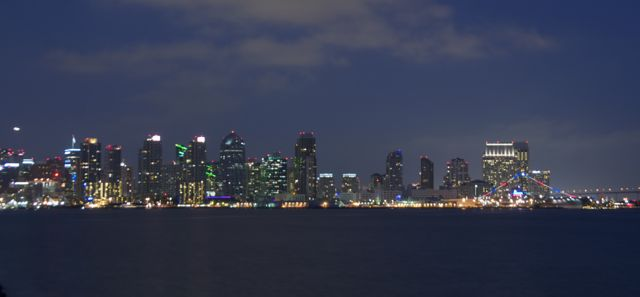
\includegraphics[width=0.5\textwidth]{sandiego}
  \caption[A picture of San Diego. Short figure caption must be \protect{$< 4$} lines in the list of figures]
{A picture of San Diego.  Short figure caption must be \protect{$< 4$} lines in the list of figures and match the start of the main figure caption verbatim. Note that figures must be on their own line (no neighboring text) and captions must be single-spaced and appear \protect\textit{below} the figure.  Captions can be as long as you want, but if they are longer than 4 lines in the list of figures, you must provide a short figure caption.\index{SanDiego}}
  \label{fig:sandiego}
\end{figure}

\subsection{A Table Example}

While in Section \ref{ssec:figure_example} Figure \ref{fig:sandiego} we had a majestic figure, here we provide a crazy table example.


%%%% TABLE 1 %%%%
\vspace{0.25in}
\begin{table}[!ht]
\caption[A table of when I get hungry.  Short table caption must be \protect{$< 4$} lines in the list of tables]{A table of when I get hungry. Short table caption must be \protect{$< 4$} lines in the list of tables and match the start of the main table caption verbatim.  Note that tables must be on their own line (no neighboring text) and captions must be single-spaced and appear \protect\textit{above} the table.  Captions can be as long as you want, but if they are longer than 4 lines in the list of figures, you must provide a short figure caption.}

\vspace{-0.25in}
\begin{center}
\begin{tabular}{|p{1in}|p{2in}|p{3in}|}

\hline
Time of day & Hunger Level & Preferred Food \\

\hline
8am & high & IHOP (French Toast) \\

\hline
noon & medium & Croutons (Tomato Basil Soup \& Granny Smith Chicken Salad) \\

\hline
5pm & high & Bombay Coast (Saag Paneer) or Hi Thai (Pad See Ew) \\

\hline
8pm & medium & Yogurt World (froyo!) \\

\hline
\end{tabular}
\end{center}
\label{tab:analysis3}
\end{table}

\end{comment}


%%%%%%%%%%%%%%%%%%%%%%%%%%%%%%%%%%%%%%%%%%%%%%%
%\chapter{Scaffolding Citizen-led Complex Knowledge Work}
\chapter{Social Computing for Complex Knowledge Work}

\begin{quote}
\emph{This dissertation explores how the following things happen. Complex work is hard. Needs learning. People do things in groups. Social computing misses learning (learning is around but not here). why your title is what it is, what that means, how you set up your arguments, and what claims your introductory chapter makes. Current online platforms (like Facebook) are built on insights from psychology about capturing people’s attention. My research instead takes a more socially responsible approach by integrating learning theory and collaboration for people to perform complex work such as generating and evaluating scientific theories. This has the potential to diversify the stakeholders and contributors to our future society.}
\end{quote}
\vspace{0.25in}

Social computing platforms have revolutionized how most people connect, communicate, and share. We increasingly connect with friends and strangers in different ways for a number of purposes. Friends and family can stay in constant touch with their loved ones. Strangers from different parts of the world discuss their ideas about their health. Increasingly, these connection opportunities have also translated to more active doing: people fund other's\'  ideas that traditional business places might balk at. Some have used social platforms to amplify their voice and bring about social changes. for instance, people in Sudan have taken down dictators [??]. By transforming how we communicate, share, and chat, social computing has become perhaps the greatest internet-fueled change of our times. 

%%interactive vis (social computing discussions) is awesome
% people can do stuff with hypotheses (test them?)
%    however, viz is hard (scientific work)
%        programming toolkits needed and impose burden (support needed to get started, reduce burden, and …)

However, the benefits of social computing are not distributed equally. While everyone has a voice, some have bigger loudspeakers than others: xx\% of most popular posts are from experts. While anyone can organize and bring changes, collective attempts to organize frequently fail. While anyone can learn from widely accessible research papers and articles, people create faulty insights from self-tracking and conspiracy theories abound. With this lens, social computing seems less transformative but rather a highly scaled up version of the offline reality of limited expertise people live in. 
% 1 to 1 link with the first para

%\subsection{Pivot to people - People can do great things but need help...}
%Well, what are people good at? What are they motivated to do? 

%People have complementary knowledge in comparison to experts and are uninfected by expert biases; these insights are drawn from lived experience, both individual and collective.

Specific to this dissertation: While social computing platforms have vastly succeeded at keeping people engaged and sharing, they barely support \textit {citizen-led enquiry}. People have strong personal motivations and contextual insights. People possess a remarkable ability to identify patterns and create theories from their experiences [??]. While most people have an amazing breadth and depth of ideas, they lack the expertise to implement these ideas. To create knowledge, they need mental scaffolds for organizing complex work, domain knowledge to compose and execute the steps, and ways to ask for help. Experts benefit from conceptual knowledge, professional training, pre-existing organizational structure for collaboration, and direct access to resources. Currently, citizens lack these resources. social computing platforms where people spend ridiculous times provide little support. 

%this is the current state --  this is the big challenge, why is it a challenge
%% however, scaling good teaching is hard - kulkarni
%     this peer thing can be helpful (evidence from small studies)
%        however, this is challenging — 2 causes
%        interfaces need to provide scaffolding 


\begin{figure}[b] 
  \centering
  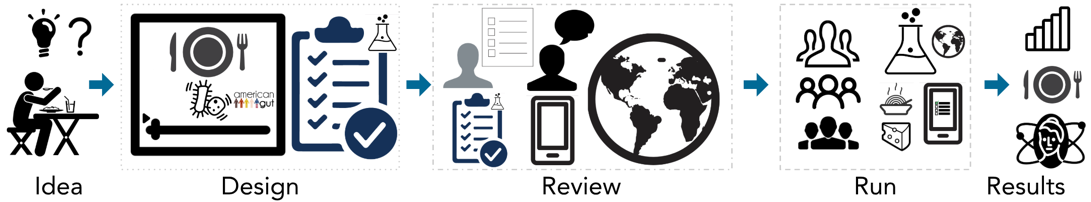
\includegraphics[width=1.0\textwidth]{figures/intro/intro-1}
  \caption[]
{The Gut Instinct platform enables anyone to transform their intuitions to hypotheses 
and then design and run experiments to test them [xx-xx]. Gut Instinct integrates 
conceptual learning embedded via short lectures and software-guided procedural 
learning to enable designing and reviewing experiments. Participants from around
 the world join experiments, follow instructions, and pro-vide data in response to 
automated data collection reminders. }
  \label{fig:intro-1}
\end{figure}

Consequently, this is unfortunate missed opportunity for both individuals and the world at large. Enabling peoplt to learn to perform personally meanignful work can help them answer their own questions. People's ideas can catalyze creating new knowledge that we are missing out on.  How might online systems support citizen-led knowledge work? 

Let''s reflect on this dual nature:  science can answer life-relevant questions but few know how to even get started. As a result, people fail to answer their questions and institutional science misses out on ideas from beyond the ivory tower. 

%one line to summarize my work -- see other intro

%two properties of classes help us - kulkarni
%this thesis leverages these two properties and provides a new class of benefits etc... 

%what helps us
%1. the scientific method is structured
%    1. even though creative and open-ended
%2. roles: people take them online
%    1. captures diversity — breadth
%    2. micro-expertise supports this explicitly 
%3. procedural learning: can teach people how to do things
%    1. captures learning — depth


This dissertation advances the design of social computing systems by integrating learning and collaboration to enable complex work such as generating and evaluating scientific theories. Over 600 people from 30 countries have self-organized to generate theories about the human microbiome and test them by running experiments. This dissertation raises the question: how can global communities create knowledge that meets their goals without waiting for experts to lead? 

Gut Instinct emodies this insight and introduces a collaborative citizen science platform for people to transform lived exes into scientific theories. 

%%%%%%%%%%%%%%%%%%%%%%%%%%%%%%
\section {People already do great things but struggle with complex tasks}

\subsection{People are awesome}
People design, build, and track to better understand and improve their health [?? dana lewis].  On numerous online fora, people share their intuitions, observations, folk theories, and even results from trying different approaches to improve their health, e.g. from simple ideas like ‘giving up drinking coffee to improve quality of sleep’ to tests and dietary approaches. People draw ideas from current research by reading and discussing papers. In many cases, these discussions are not just anecdotal but also derive from state-of-the-art scientific work. In some cases, people contribute back to scientific work as well.How can social computing platforms effectively enable people to do more personally meaningful work built upon their experiences and insights?

People’s curiosity, needs, and possibilities to do useful work is endless; however, traditional online systems don’t support them. Online fora encourage long, rambling discussions. Online learning provides conceptual lessons but people drop out and these are not linked to people’s needs.While learning resources like MOOCs abound, they hardly meet the need: many drop out, the lectures focus on conceptual knowledge, and lack the feedback needed to perform open-ended creative work. We know little about integrating learning resources and social computing affordances are far from each other. Moreover, currently both learning and work are not personal; can we change this? Lack of appropriate "learning abstractions" make complex work unrealistic.

The goal is to create environments for learning and collaboration through complex, personally meaningful work.

%%%%%%%%%%%%%%%%%%%%%%%%%%%%%%%%%%%%%%%%%%%%%%%%%%%
\subsection{Challenge: People' don't know what to do and how to do it}
Citizens have a different background than professional scientists; they have unique
 personal experiences but lack the years of domain training. Two major issues in 
enabling complex work on the internet are (diversity and scale?) 
quality of individual contribution and managing overall contributions from the crowd.
We desire social computing techniques that reliably enable a wide variety of people to 
contribute more than they naturally could and that manage the dependencies among
 a large set of tasks.

To create computational systems that leverage their strengths and mitigate the lack of training, this dissertation 
focuses on domains where the science is nascent, highly contextual, and personally motivating.
 Synthesizing the crowdsourcing literature and my experience highlights three challenges: 
poor signal-to-noise from crowds due to lack of training; inefficient collaboration without 
careful attention; and poor results (or no results at all) unless experts lead. 

To address  these concerns,  this dissertation introduces and evaluates peer production architectures 
and procedural learning.

\subsection{Scientific experimentation: An instance of complex knowledge work}
%here''s an example: experimentation 
Supporting complex knowledge work has been a challenge for Human Computer Interaction
 research (make specific). For instance, many people are interested in understanding and 
improving their health. Millions of peple from all over the world share their insights. 
Can't they run experiments for these?

Scientific experimentation features technical requirements and contextual choices 
that are inscrutable for a lay individual yet necessary for success [??]. While 
professional scientists and commercial ventures run experiments every day, with 
notable exceptions [??], empirical papers from non-professionals are 
vanishingly rare. This biases the questions asked, studies run, and knowledge 
created [??]. People have questions about their health, but lack the expertise 
and resources to scientifically investigate them. Broadening the pool of 
experimenters could help people investigate their curiosities, develop solutions 
to improve health and performance, and assist institutional researchers.


\textit{People lack the expertise to know what to do and how to do it.}. 
Success with complex creative activities requires procedural
knowledge (how to do things) in addition to conceptual
knowledge (facts). While many resources offer facts, procedural
learning is often ignored.The converse also holds, and much more often: novices are also
“uninfected” by all the knowledge that enables experts to
innovate.Sometimes, having a different background than experts can
be beneficial. Shared knowledge is great when it’s right, but
blocks progress when wrong. When false assumptions limit
experts, at least some novices are likely to be “uninfected”.
For example, GalaxyZoo volunteers discovered ‘green pea’
galaxies overlooked by scientists who mistakenly assumed
the green hue was merely an imaging artifact [54]. 


% kulkarni -- "This assessment requires bothcommon-sense knowledge to understand student work and the expertise to assess tacit criteria such as “well-designed” or “well-modularized” that cannot be completely articulated. Indeed, teaching such tacit criteria is an important goal in open-ended domains like design"


\textit{People lack a professional network to improve their work}. 
Furthermore,  how do people ask others for help? Who do they reach out to?

People are connected online and collectively have access to many resources.
In a large distributed community, there’s often someone who happens to 
have important relevant knowledge, usually drawing on a relevant but 
distant domain. Such distributed efforts are a type of lead-user innovation [31]. 
Having many people work on the same problem increases the odds that 
one will break through. Drawing on secondary expertise as inspiration can
 be an important agent of creativity because almost by definition, the 
combination is rare [10]. %Open \& crowd innovation builds up on contributions
 by diverse online participants, and a ‘bubbling up’ process for strong ideas [56].

While many hands make light work, novices need clear contribution opportunities. 
The crowdsourcing literature offers many good verification approaches for tasks 
with clear right or wrong answers – like whether two images represent the same 
product or what street number is written on a sign. However, verifying knowledge
 work necessitates a different approach because it requires making 
situationally-appropriate choices. 

%%%%%%%%%%%%%%%%%%%%%%%%%%%%%%%%%%%%%%%%%%%%%%%
\section{Thesis Statement and Contributions}
\noindent This dissertation investigates the question: how to enable people to perform personally meaningful work otherwise beyond their expertise? Underlying these investigations is the thesis:
%"My thesis statement is"
\begin{quote}
\emph{Providing task-specific guidance in social computing enables personally meaningful \& useful scientific work}
\end{quote}

This dissertation\textquotesingle s primary contribution is the idea of intergrating learning in social computing to enable groups of novices to perform complex, creative activities. The thesis achieves this integration by building a sequence of interactive prototypes that enable people to collaboratively generate and test hypotheses. In the process, the prototypes divide complex work into distinct activities: self-sourcing the design and crowdsourcing people''s inputs and data. Every prototype advances social computing further as a domain for deep, personally meaningful work. Beyond introducing learning abstractions, this dissertation carefully designs the affordances, support, and system to enable different users for different needs. 

 %To realize this idea, 
This dissertation makes three types of contributions: theoretical perspectives/techniques, real-world systems, and outcomes including empirical results, systems lessons, and dataset (Figure \ref{fig:contributions}). 

%%%%%%%%%
\subsection{Theoretical  Techniques}
Improving  work quality in social computing suggests deepening individual contributions and broadening participation by providing different contribution mechanisms.The former requires better learning tools and the latter requires better collaboration tools and dependency management. Consequently, this thesis' theoretical contributions include 1) principles to integrate guidance for complex tasks, and 2) ways to divide complex tasks into multiple roles or affordances.

%“..adapts and extends techniques from xxx” -  arvind

%system-led learning vs people-led
Traditional systems think of knowledge as being provided by the people, while we being the knowledge from the system itself.

%todo-introduce the learning and collaboraiton taxonomy here
\begin{figure}[b] 
  \centering
%  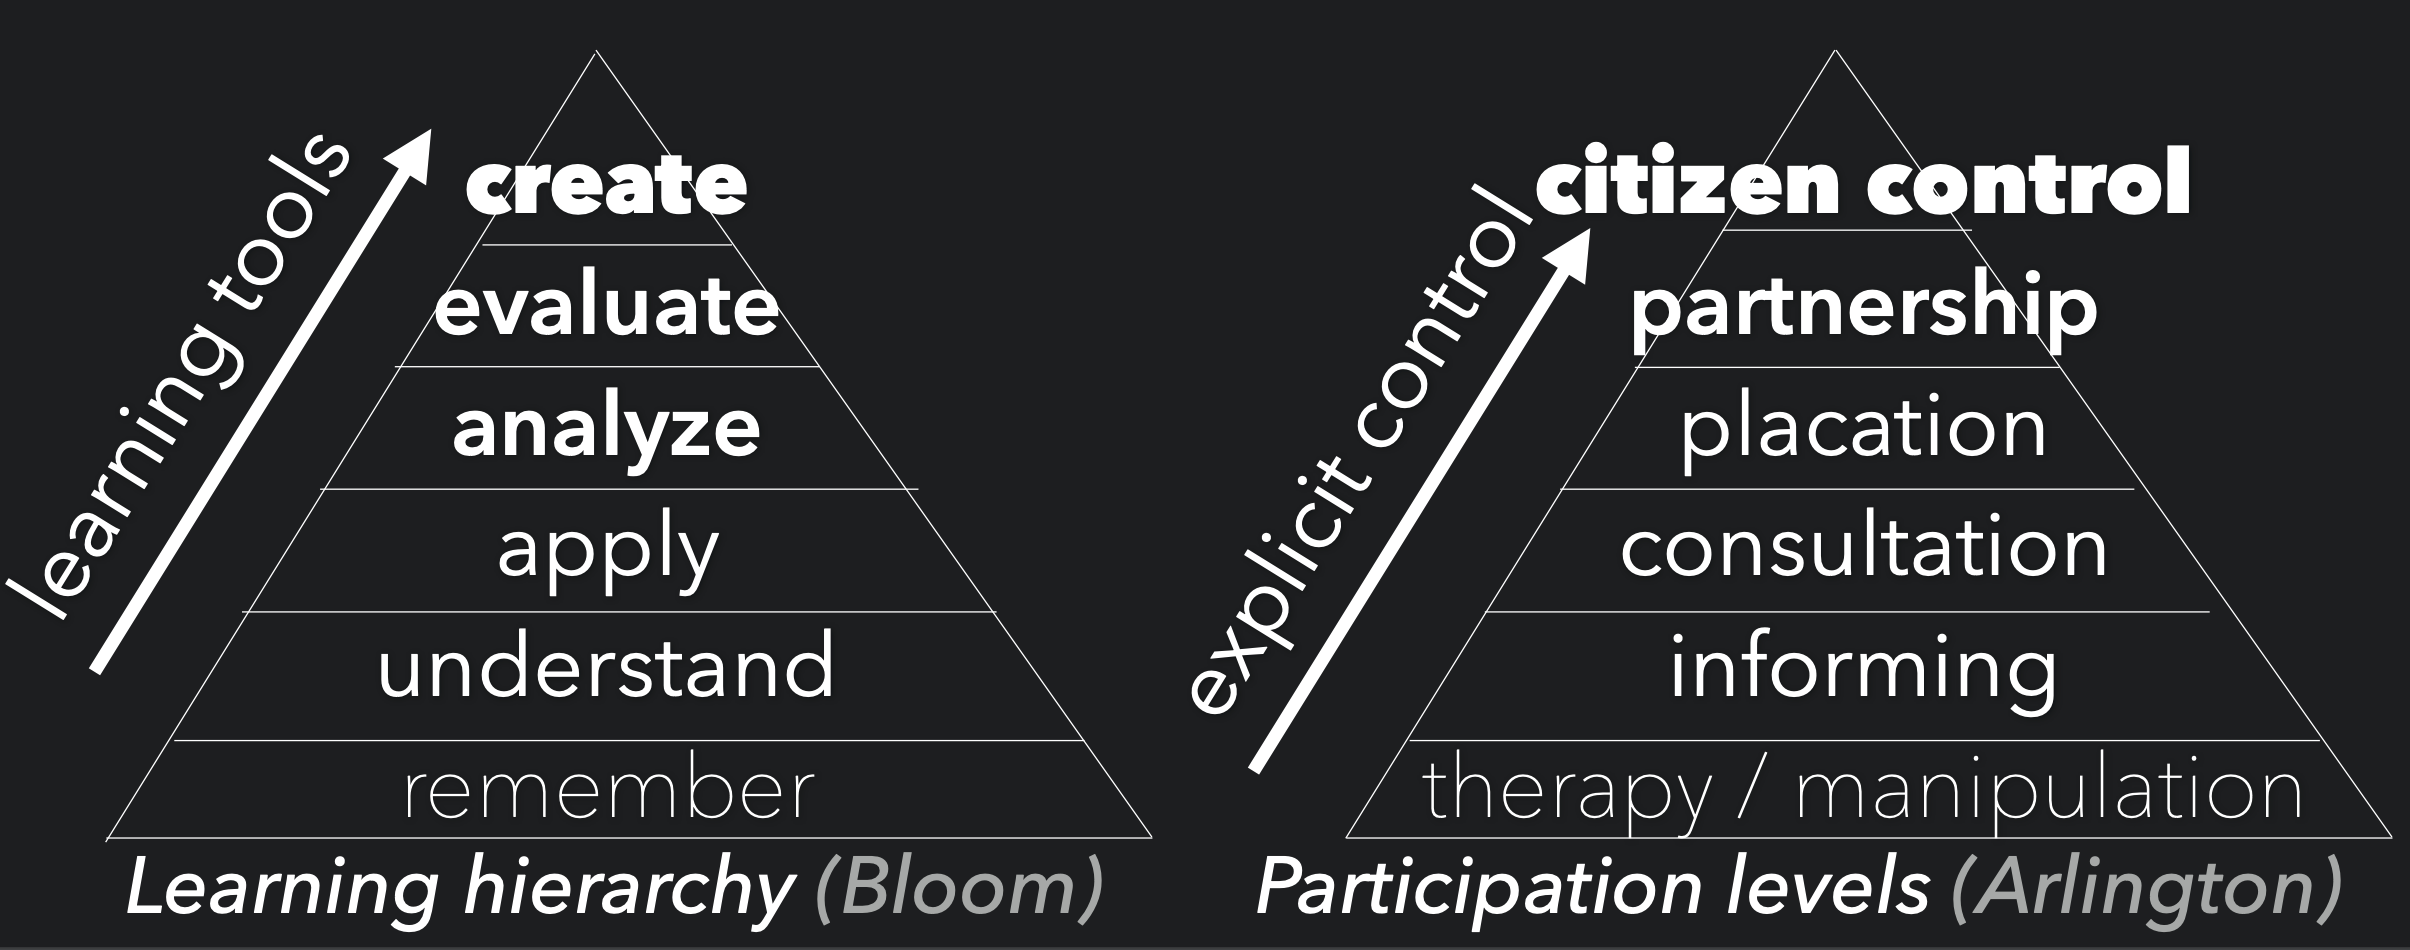
\includegraphics[width=1.0\textwidth]{figures/intro/intro-taxonomy}
  \caption[]
{Drawing from Maslow's hierarchy of learning and xx's hierarchy of contribution}
  \label{fig:intro-taxonomy}
\end{figure}

% come up with principles myself
%figure about conceptual and procedural learning 
\textit{Principles to integrate learning in social computing}: Learning broadly comprises conceptual (declarative) and procedural knowledge. Conceptual learning is where people learn what something is, learn about its features; this is a big part of current teaching. Typically, such learning is tested with test questions. In contrast, procedural learning teaches the {\it how} of things. How do you do x, y, or z.  Concpetual learning is useful when xxx while procedural learning is more useful when yyy.

To make useful contribution, people need to have a good working model of both the concepts and procedures for an activity. This dissertation enables this in two ways: 1) reifying conceptual bits in the software, and 2) providing procedural guidance with examples, checklists, and templates. Building on Maslow''s hierarchy~\ref{??}, it aims to push learning more up.

\textit{Principles to decompose Complex work to f(people, community, \& machines)}
% figure -- def needs one -- based on strengths and weaknesses
%fig - present a stack of things
The individual, groups of people, and machines possess complementary strengths. Individuals have personal motivation to do something; their lived experiences provide ideas that might be potentially novel. Groups of people might not be as motivated but might be willing to help by providing another set of eyes and complementary knowhow and insights from lived expeirences; they can help check biases with the diversity of their lived experiences. But since they are not as motivated, maybe limited affordances would be useful. Computers can implement things consistently to reduce biases but they cannot interpret open-ended instructions fairly in different contexts the way people can.  (todo- fix this to crisp english writing) (see slide deck)

Given these complementary strengths and limitations, this dissertation 1) begins every task with a heavy-handed implementation by an individual personally invested in that idea, 2) improves it with others'' feedback, and finally, 3) runs the idea with the help of automated software. For all these steps, the system manages the interdependencies beneath the sheets to reduce pressure on people. Building on xx's hierarchy~\ref{??}, it aims to push collaboration more up.

The efficacy of these techniques is borne out over multiple deployments. All these techniques have been put in systems as interfaces, intelligent backends, and so on... \\

%\begin{figure}[t!] 
%  \centering
%    \includegraphics[width=1.0\textwidth]{figures/img/intro/1-contributions}
%  \caption[Contributions of this dissertation]
%{Contributions of this dissertation including empirical results theoretical perspectives/techniques, real-world systems, and multiple outcomes}
%  \label{fig:contributions}
%\end{figure}

\subsection{User Interface and System Design}
%User interfaces and system design for efficient implementation
%figs needed to explicate 

While guidance techniques and role differentiation provide the building blocks, they are by themselves insufficient for useful higher-order collaborative work. These techniques need to be baked in simple, interactive interfaces. Multiple challenges show up for this question. First, the internet is a diverse community and have varying levels of expertise. So, the things need to be understandable to all. Second, people might have poor models of thiking about stuff and might frame their ideas and intuitions in weird ways.Third, the interface should make it easy to keep moving and get unstuck.  Too much information might make people struggle, so we need UIs for focused collaboration. 

This dissertation by bakes the techniques in the user interface  and by building a backend that is based on the principles of x, y, and z.

%System contributions
Gut Instinct  introduces a collaborative citizen science platform for people to transform lived exes into scientific theories. Gut Instinct frames the task of hypothesis-testing as a crowdsourcing problem, develops techniques and platform that supports different roles with just-in-time learning, and provides efficient backend support to automate simple tasks.

Gut Instinct divides multi-party collaboration into complementary tasks and supports them using different contribution mechanisms (like adding a question, editing a response) and roles (like experimenter, reviewer, participant). This provides people the flexibility to choose how much they’d like to contribute. Finally, Gut Instinct automatically manages multiple activities to reduce 
bias and experimenter/participant workload,such as randomized placement of 
people into conditions, maintaining anonymity, and collecting and cleaning data.


Take for instance, the state diagram — the edges represent what people need to do 
Roles Support via Just-in-time Skill Acquisition:  People take different roles--write up form galileo

%%"Furthermore, adding location information to photo collections is by itself insufficient for scenevisualization: we also need intuitive, interactive interfaces for exploring these scenes. There are several challenges faced in the design of such interfaces. First, unlike with Google Street View, where photos are taken at regular intervals, personal or Internet collections are typically an unstructured soup of photos. Nevertheless, the navigation controls should still be intuitive and exhibit regularity. Second, such controls should make it easy to find and explore the interesting parts of a scene, particularly for tourist sites."

%%%%%%%%%%%%%
\subsection{Outcomes}
\subsubsection{Empirical Results from Real-world Deployment}
expertise: limited; diversity: different countries; scale: some

\subsubsection{Dataset}
1. repo of hypotheses with rating
2. repo of experimental designs
3. ...

\subsubsection{Impact}
344 volunteers from 27 countries created 399 hypotheses about their health and the gut microbiome. Remarkably, microbiome scientists rated a fifth (75) of these hypotheses to have a scientifically valuable insight about a topic not covered by existing published work. Volunteers fleshed out 60 of these hypotheses into complete experimental designs. My entire work (code + data) is open source so others can edit, build, and experiment.

This dissertation has also enjoyed sufficient support in multiple research communities: Innovation researchers at MIT, online and offline fermentation and self-tracking communities, and citizen science groups. Finally, parts of the system have been taught in classrooms including CSCI 499: (Computing for Social Good) at USC. 

This work explores how online learning and process training systems, combined with
peer collaboration, can help people learn similar skills that
can be useful in scientific and design domains.


%%%%%%%%%%%%%%%%%%%%%%%%%%%%%%%%%%%%%%%%%%%
\section{Dissertation Roadmap}

%%%%%%%%%%%%%%%%%%%%%%%%%%%%%%%%%%%%%%%%%%%%%%%%%%%%%%%%%%%%%%%%%%
%todo- “we” refers to the set of authors…  -- see arvind

My dissertation demonstrates how we might draw on people’s diverse background knowledge, interest, and micro-expertise to expand scientific knowledge and push it in new directions. More specifically, the Gut Instinct platform that I have built instantiates these ideas enabling participants of the American Gut Project (the world’s largest crowdfunded citizen science project) to generate and experimentally investigate hypotheses (Figure 1). 

This dissertation creates the opportunity of harnessing humanity\textquotesingle s collective efforts to accomplish great goals.
s


"double quotes"


%The techniques make the idea concrete; the system operationalizes the techniques and makes them work; and the outcomes discuss the successes and failures of our approach.

%to people for them to perform personally meaningful work.
%My research prototypes collective systems for large-scale problems.
%Worldwide, people use online health fora to share insights and look for answers
%Iin short, to push people towards actively testing their ideas rather than just sharing them?  whether drinking kombucha really changes the gut constitution? In the absence of support and guidance, how can people do more? . 

%%1. novice-led
%    1. no experts
%    2. with other novices 
%2. personally meaningful 
%3. techniques
%    1. expert work to social computing 
%        1. ways to do that
%4. output
%    1. create new knowledge 

\chapter{Related Work}

\begin{quote}
\emph{This chapter summarizes research in citizen science, lead-user innovation, and social computing that inform the design of systems in this dissertation}. Citizen scientists have successfully solved expert-defined problems as sensors or algorithms. However, public involvement in scientific endeavors fail to provide a true participatory experience that is citizen-led and personally meaningful. Lead-user innovation provides a complementary setup. Lived experience, a tight feedback loop, and strong personal motivation enable people to create different and sometimes better products than experts; however, lead users rarely have access to training, conceptual knowledge, and pre-existing organizational structure for collaboration. Finally, social computing and crowdsourcing platforms support sharing potentially novel ideas but converting these to actionable plans requires expert guidance. This dissertation provides ways to integrate learning in social computing to enable deeper contributions from citizen scientists and lead users without expert involvement.
\end{quote}

%Professionals have the advantages of training, conceptual knowledge, and pre-existing organizational structure for collaboration and support; however, lead users rarely have access to such systematic support.

\begin{figure}[!h] 
  \centering
  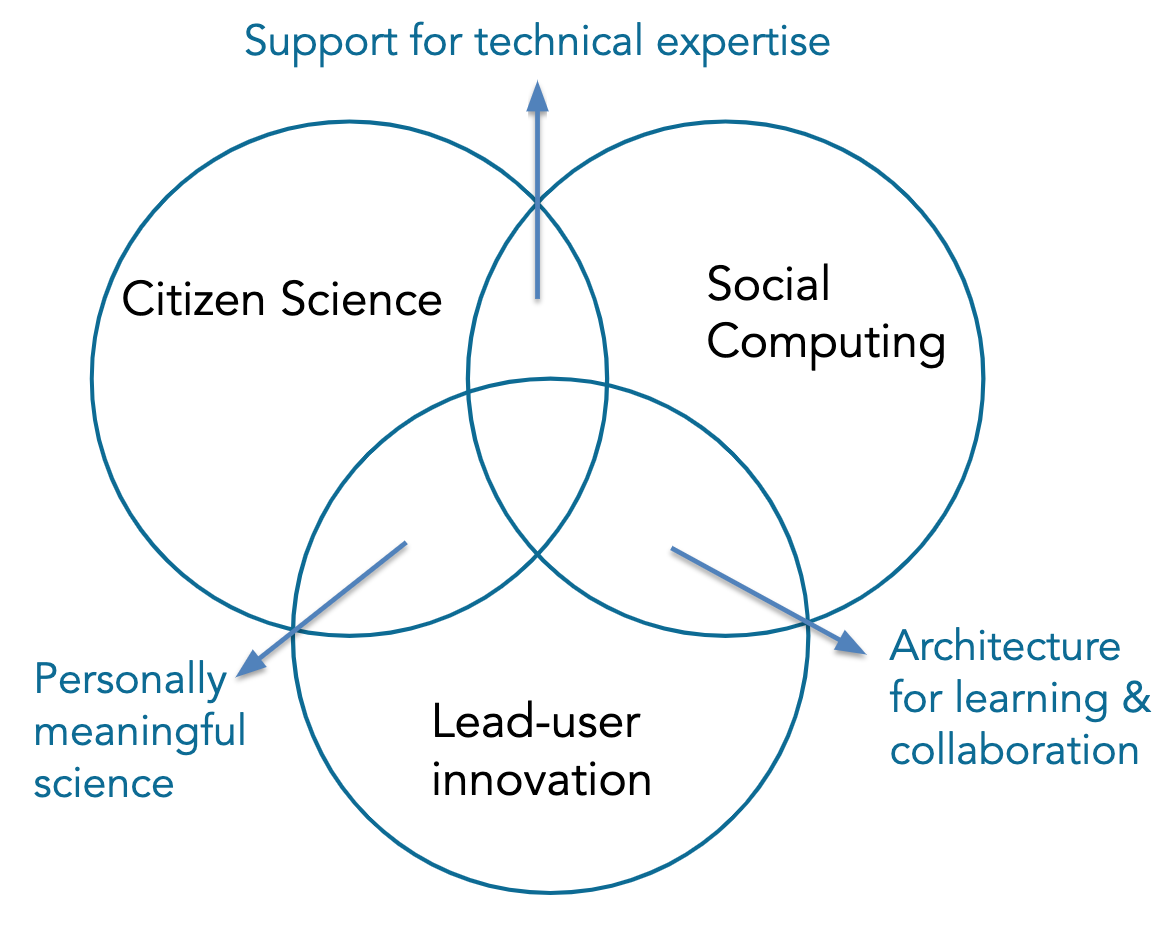
\includegraphics[width=0.6\textwidth]{figures/2-related/venn.png}
  \caption[]
{This dissertation draws from and contributes to citizen science, lead-user innovation, and social computing\index{related-1}}
  \label{fig:related-1}
\end{figure}

\vspace{0.25in}

%So, we find that there are three main challenges for citizen science: 1) make it personally meaningful, 2) deepen the contributions that citizens can make. 3. 1. Improve the quality of poor contributions — and improve the quality of max contributions     1. — hockey stick curve 
%%%%%%
\section{Science is increasingly networked but misses people’s lived experience }
Science is increasingly networked, multidisciplinary, and
open~\cite{Pandey2017}. For instance, \textit{LIGO}’s pathbreaking discovery of
gravitational waves brought together over 100 researchers
from over 100 institutions across 18 countries (ligo.org/about). 
Scientists increasingly share data and results faster (arxiv.org). 
Large scientific projects, like the \textit{Human Genome Project}, 
took to agile science by sharing methods, data, and insights to 
collaboratively speed discoveries. Scientists also form global 
collaborations to accelerate research in nascent scientific domains, 
like the Earth Microbiome project (earthmicrobiome.org).
At its best, institutional science has benefitted immensely
from large-scale global collaboration. Complementing this success,
many online projects enable people to help scientists~\cite{Nielsen2012}: annotating 
scientific papers~\cite{Good2013}; labeling galaxies~\cite{JordanRaddick2013}; and providing microbiome 
samples~\cite{McDonald2018}, CPU cycles (worldcommunitygrid.org), or personal data (openhumans.org). 
Efforts to further expand participation in scientific research are bearing fruit: \textit{Lab in the Wild} 
recruits anyone with an internet connection for behavioral studies~\cite{Reinecke2015}; and \textit{All of Us} aims 
to recruit one million Americans from all strata of society (allofus.nih.gov). Such collaborative efforts from experts 
and citizens suggest a new model for scientific work.

Often, when citizens participate in science, it is as \textit{embedded sensors} that 
are aggregated by experts. Public involvement in scientific endeavors continues
to be largely limited to performing tasks just beyond the reach of computers.
A classic example is \textit{Audubon}’s Christmas bird count, run since 1900
~\cite{Audubon2016}. Online examples include reporting flower blooms in
\textit{Project Budburst}~\cite{BoulderColorado2016}; recording wildlife activity~\cite{Faridani2009a};
identifying galaxies from satellite imagery in \textit{GalaxyZoo}~\cite{Zooniverse2007}; 
and biochemistry games: finding protein structures in \textit{Foldit}~\cite{Cooper2010}, 
synthesizing RNA molecules in \textit{EteRNA}~\cite{Lee2014}, and aligning 
nucleotide sequences in \textit{Phylo}~\cite{Kawrykow2012}. Distributed 
data contributions from people around the world—browsing online~\cite{Coviello2014}, using activity trackers, and joining scientific projects—have enabled valuable insights on topics including 
obesity~\cite{Althoff2017}, aesthetic preferences~\cite{Reinecke2014a}, sleep~\cite{F.lux2019}, and the human microbiome~\cite{McDonald2018a}. At their
best, these citizen science platforms yield novel insights.
For example, \textit{Foldit} players discovered protein structures
that helped scientists understand how the AIDS virus reproduces~\cite{Coren2011}. Why have such collaborative efforts succeeded?


%Different people provide different expertise that can vet claims and  fix mistakes~\cite{kane2009s}.
Collaboration benefits creativity when it brings different
 perspectives that build on each other; it impedes creativity (or worse, causes regression) 
when—through groupthink—it spreads biases rather than removing them~\cite{starbird2014rumors}. 
A humbling example of the power of fresh eyes: volunteer citizen scientists identified a new class of 
galaxies (\textit{green pea} galaxies) after researching green blots on \textit{Galaxy zoo} images; 
experts had dismissed these images as apparatus error~\cite{cardamone2009galaxy}.
This volunteer-led discovery demonstrates the need for fostering independent perspectives 
while simultaneously cultivating sufficient knowledge for meaningful domain contributions. 
Such collaboration requires strategic isolation: roviding just enough scaffolding to keep 
biases independent, while not stifling original ideas for bottom-up knowledge creation.

%This dissertation draws on the idea of people using  cognitive surplus to collaboratively answer scientific questions~\cite{Bonney2009}.


%%%% - where does this go
%Such bite-sized contributions is not without reason—a lot of
%scientific work requires deep conceptual knowledge and 
%training in scientific process to perform useful work. Most
%citizens lack the time, resources, and motivation to develop
%narrow, unique skillsets. Expanding the depth and breadth of work 
%performed by citizen science communities would be useful.

%\subsection{Citizen Scientists: From Collectors to Experimenters}
\subsection{Opportunity: Can people be scientists rather than just sensors?}
Citizens have successfully solved expert-defined problems as sensors or algorithms with a 
row-filling model of contribution.
In the quest to get people to track, measure, accumulate, or
sort both digital and analog data, citizen science has overlooked the massive 
opportunity of leveraging people’s unique advantages: our skills as reflective, 
creative thinkers who generate theories about the world, including ourselves.
People can offer more than just their data and perceptual
skills: they create theories, right or wrong, about a wide
range of topics including emotions~\cite{Johnson-Laird1992a}, motivation~\cite{Markus1991}, or
diet. These may be observational theories~\cite{Kempton1986}, folk theories
passed in a family/culture across generations~\cite{Gelman2011}, or ideas
brainstormed in online communities~\cite{23andme2016}. Perhaps, these intuitions 
can provide a starting point for independent, participatory experience that also assists the scientific community.

When are such personal experiences worth paying attention
to? For every intuition proven right, many more may be
closer to snake oil — e.g., the widespread belief in the utility
of probiotics despite limited evidence~\cite{Bonifait2009}. The global internet
increases the proliferation of both powerful and questionable
ideas: sharing speculation is fast while evaluation remains
slow. Moreover, people develop intuitions of cause and effect
that may or may not be correct. Current online forum
designs prioritize discussion — sharing personal details in
long, free-flowing text — over structure, succinctness, learning,
and potential scientific utility~\cite{Thomas2002}.

Advances in precision medicine have demonstrated the need
to engage people in uncovering and sharing insights~\cite{Aronson2015}. People
are highly motivated to improve their health outcomes,
more so if they suffer from a condition that severely affects
their quality of life, naturally forming communities. For example,
patients from the Amyotrophic Lateral Sclerosis
(ALS) community on \textit{Patients Like Me} (patientslikeme.com)
organized a study to track effects of Lithium on their symptoms
~\cite{Wicks2011}. This is not surprising; lead users excel at tackling
\textit{need-intensive} problems where they can use their lived
experiences to identify problems, try solutions, and readily
observe the effects~\cite{VonHippel2005}. Other organized communities like
\textit{Quantified Self} hope to uncover lifestyle patterns that may
improve their productivity and health outcomes. The word
‘self’ belies the fact that such movements are highly collaborative:
amateurs frequently share experiences and invite
feedback on online fora (patientslikeme.com) and blogs
(ibsgroup.org). Millions follow these ideas and some incorporate
these intuitions in their lives. What kinds of scaffolds
and structure may help people generate better ideas and implement them as actionable plans that
enable researchers to identify promising insights?

%How can people expand their insights into scientific work?

Most scientists develop their skills through an apprenticeship-
based graduate school experience. Apprenticeships emphasize
hands-on experience with individualized, taskspecific
feedback~\cite{schon1984reflective}. Scientists possess a wealth of declarative
knowledge about their domains (e.g., how to set up a
randomized controlled trial), and also procedural knowledge
—some narrow, some broad —towards getting things done
(e.g., improving fMRI signal intensity by having participants
consume cocoa beforehand~\cite{Francis2006}). This dissertation explores how
online learning and process training systems, combined with
peer collaboration, can help people learn similar skills that
can be useful in scientific domains.
%So, we find that there are three main challenges for citizen science: 1) make it personally meaningful, 2) deepen the contributions that citizens can make. 3. 1. Improve the quality of poor contributions — and improve the quality of max contributions     1. — hockey stick curve 
%WOULDN'T IT BE GREAT TO HAVE PEOPLE DESIGN AND RUN EXPERIMENTS AS AN INSTANCE OF COMPLEX SCIENTIFIC WORK
%Link to lead users -- people already doing personally meaningful work.. 

%%%%%%%%%%%%%%%%%%
\section{Lead users Succeed When They Know What to Do and How to Do It}
%“Lead users are rarely experts by themselves. They are novices who find themselves at the right place, with the right tools (that they might have created themselves), and who have the courage to follow through.” Lead users have created different—and in some cases better designs— than experts. 

%examples: UN example (see eric vh)

Lead-user innovation is both an inspiration and an application area for this dissertation. Lead users are
users of a product (or service) who experience advanced needs unmet by existing products~\cite{VonHippel2005}. The
power of lead-user innovation is that lived experience, a tight feedback loop, and strong personal
motivation can yield different and sometimes better products than experts [32]. For example, diabetes
patients have improved insulin delivery [47] and snowboarders have improved their binding
ergonomics. Lead users also collaborate online to build software
(github.com), create novel hardware \& reference designs
(openaps.org), and share personal data (quantifiedself.com,
openhumans.org). Some go further still, e.g., the transcranial
direct-current stimulation community draws ideas from scientific
papers to attempt self-experiments (reddit.com/r/tDCS). In a few exceptional cases, lead users have authored
scientific papers, e.g., Open Artificial Pancreas creator
Dana Lewis discussed the benefits and challenges of first-generation
automated insulin delivery at the 2016 American
Diabetes Conference~\cite{DanaLewis}.

Why do people do this? Curiosity, personal learning, and social
comparison are three reasons~\cite{Reinecke2015}. A massive interest in
personal genomics (over 1 million 23andme participants)
and the human microbiome (13,000 \textit{American
Gut} participants) demonstrates people’s yearning for self-understanding.
Users of these platforms send data, answer survey questions,
and discuss on fora. Some even use online lectures to understand
concepts of genes, phenotypes, and microbiota~\cite{23andMe2017, Knight2016}. 

\subsection{Opportunity: Providing lead users the expertise to tackle complex knowledge work}
Sometimes, having a different background
 than experts can be beneficial. Shared knowledge is great when it’s right, but blocks progress
 when wrong. When false assumptions limit experts, at least some novices are likely to be 
\textit{uninfected}. The converse also holds, and much more often: novices are also uninfected
by all the knowledge that enables experts to innovate. Lead users have an advantage when the key ingredient is experience intensive; experts retain the
advantage for \textit{solution-intensive} innovations [32]. In a large distributed community, 
there’s often someone who happens to have important relevant knowledge, usually 
drawing on a relevant but distant domain. Having many people work on the same problem 
increases the odds that one will break through. Drawing on secondary expertise as 
inspiration can be an important agent of creativity because almost by definition, the
 combination is rare~\cite{Boden2004}. 
%For example, GalaxyZoo volunteers discovered ‘green pea’ galaxies overlooked by scientists who mistakenly assumed the green hue was merely an imaging artifact~\cite{Tinati2015}. 

Community-driven approaches to understand personal
health and well-being largely reside outside the realm
of institutional science and medicine. While some fads and beliefs are 
questionable at best, on occasion communities
break new ground that may provide widespread value,
such as fecal transplants to alleviate \textit{Clostridium difficile} infection
symptoms~\cite{Brandt2012}. Some doctors recommend that patients
track their symptoms and reflect upon them to find
insights. Putting people in charge can help them find significant
relief for ailments like chronic migraine~\cite{Gawande2017} and provide
researchers and clinicians with useful patient data
(smartpatients.com). Insights from N\Hair=\Hair1 studies have helped
crack scientific puzzles about the working of the mind~\cite{V.S.Ramachandran1998},
heart, and microbes~\cite{Weisse2012}. 

Personal needs and challenges can be highly motivating but performing complex work still requires multiple rounds of trial and error. 
People need to know the genre of work and implement it correctly.  Professionals have the advantages of training, conceptual knowledge, 
pre-existing organizational structure for 
collaboration and support, and direct access to resources. Lead users either seek these resources from others or need to create them. 
Providing a correct and complete model for complex, structured activities might reduce efforts and improve the quality of results.
This dissertation reduces the gap between lead users' ideas and implementation by providing templates for 
genre work using just-in-time training and a collaboration platform to find others. This dissertation focuses on enabling people transform their idea to a controlled experiment as opposed to 
self-tracking or informal iteration which is the focus of most current citizen-led work in health.

\subsection {Case: Scientific experimentation is difficult}
While public contributions have supported institutional science; it’s rare for citizens to design
their own experiments. A number of health and behavioral research projects enlist citizens as helpers (e.g., \textit{HabitLab} [43]). 
\textit{CivilServant} enables online communities’ 
moderators to test policy ideas; moderators share these ideas with researchers who transform 
them to study designs [51]. Through the \textit{PatientsLikeMe} website (patientslikeme.com), citizens 
and scientists created a study investigating whether consuming lithium alleviated ALS symptoms [64]. 
While an initial scientific study had provided positive benefits, both this citizen science study and 
a subsequent university study did not find benefits. \textit{Tummy Trials} asked 
participants to generate health questions, introducing a protocol for self-experimentation 
combining ideation and self-tracking [36]. In all these cases, citizens rely on experts to provide sound experimental design.

Why is experimentation hard?  Despite a predetermined goal and a formalized process, experimentation
requires making situationally-appropriate decisions. A dependent variable may produce crisp
numbers but feedback on the experiment design itself is more multifarious. Good experiment
design is inherently user centered: how will participants interpret the instructions? Experiment
designers need awareness of others’ interpretation of their ideas and asks. Feedback and iteration
might be key to creative success, especially for novices. Providing feedback on experiment
designs requires knowing the success criteria and how to
help improve.  Feedback can be provided by experts~\cite{dow2012shepherding, schon1984reflective}, peers~\cite{Boud1995, Kulkarni2015b}, software~\cite{Dantoni2015, Head2017}, or even oneself~\cite{Boud1995,schon1984reflective}. While feedback from novices can
potentially improve both structure and content, it can also emphasize superficial issues over the
underlying structure~\cite{chi1981expertise}. Finally, successfully running an experiment
requires managing multiple processes such as random
assignment, anonymizing participant details, and sending
instructions and reminders for data collection.

%%%%%%%%%%%%%%%%%%%%%%%%%%%%%%%%%%%%%%%%%%%%%%%%%%%%%%%%%%%%%%%%%%%%
%But to understand that let's look at social computing ideas...

\section{Social Computing and Crowdsourcing Architectures for Complex Work}
Canonical crowdsourcing breaks larger tasks into microtasks; algorithms specify the division,
dependency, and agglomeration activities while workers perform small tasks supported by task-specific
guidelines~\cite{kittur2012future}. Leveraging existing expertise is one approach for complex knowledge work. One strategy
directly employs experts’ just-in-time feedback to improve crowd work~\cite{dow2012shepherding}. Workflows manage
experts for open-ended work like developing interactive prototypes~\cite{Retelny2014}. 
\textit{Flash Organizations} uses automated hiring, a hierarchy with a central leader, and optional 
team leaders for collaborative projects like product design~\cite{Valentine2017}.
Another strategy creates roles that enable more experienced crowd members to orchestrate
the work. \textit{Ensemble} supports leaders in guiding and constraining crowd 
contributions~\cite{Kim2014e}. Role-based approaches confer three benefits: 1) clean 
delineation of responsibilities improves chances of task completion, 2) clustering similar tasks 
reduces overhead and increases consistency; 3) people can decide their contribution levels. 
However, experts are expensive, in short supply, and sometimes prone to groupthink. 

Carefully-constructed interfaces can aid novices with task-specific expertise to solve problems 
that only experts previously could. \textit{Foldit} introduced 3D game for specifying low-energy protein 
structures via direct manipulation~\cite{Cooper2010}. Making a challenge visually salient is an 
effective way to on-board novices. For tasks that don’t have as a crisp visual analogue as protein
folding, people need better conceptual support. Prior work has explored collaborative hypothesis generation and testing on pre-existing data sets
~\cite{luther2009pathfinder,willett2011commentspace}. This dissertation offers a 
complementary contribution: enabling citizens to generate data on topics of personal interest.

One way to make complex tasks manageable is to divide them into distinct phases. 
Touchstone demonstrates the power of a semi-automated workflow integrating experiment 
design, testing, and analysis~\cite{Mackay2007}. Crowdsourcing has similarly innovated by 
creating distinct phases: break larger tasks into microtasks; algorithms specify the division, 
dependency, and agglomeration activities while workers perform small tasks supported by 
task-specific guidelines~\cite{lasecki2012real}. From these systems, our work draws the 
idea of dividing experimentation into multiple tasks—some self-sourced, others 
crowd-sourced; and introduce just-in-time domain expertise to perform these tasks. 

 
%How might groups of novices perform complex work like experimentation?
%Systems like Foldit and EteRNA powerfully show  how carefully-constructed interfaces provide
%novices with the task-specific expertise to solve problems that only experts previously 
%could~\cite{Cooper2010, Lasecki2012, Lee2014, Zooniverse2007}.

%%%%%%%
%%building up solution space - more work
\subsection{Learning resources at the right time}
Providing just-in-time supports, step-by-step instruction, and showing helpful supportive
 information are core ideas in instructional design~\cite{Kirschner2008}. Crowdsourcing 
systems leverage interactive guidance for specific tasks. For example, \textit{CrowdLayout} and 
\textit{Cicero} provide guidelines and static rules that workers use these to reason about their choices
 and improve network layouts~\cite{chen2019cicero, Singh:2018:CCD:3173574.3173806}. 
Others like \textit{CrowdSCIM} and \textit{Crowdclass} scaffold pre-task interventions~\cite{Lee2016,wang2018exploring}. 
While learning resources are distributed across the internet, they are rarely integrated with the task. 

Creative, open-ended work has rich pedagogical value. Online work, like 
online learning, requires appropriate scaffoldings, such as rubrics
~\cite{Boud1995, Kulkarni2013peer}, decision trees~\cite{Lee2016,Yu2006}, 
tutorials~\cite{Andersen2012}, and quick expert guidance~\cite{dow2012shepherding}. 
Similar to general critique of pure discovery learning~\cite{Mayer2004}, simply 
asking participants to \textit{figure it out} would be poor pedagogy. Hence, this dissertation
introduces a guided discovery learning approach as Mayer advocates: expert-curated 
learning materials help participants start, with discovery following. Such integration 
offers a problem-based learning experience with context and 
motivation for the material students learn~\cite{Savery1995}. In principle, these 
real-world problems also provide a yardstick for measuring learning. 

This dissertation introduces support during the task itself for those with little-to-no mental model of the knowledge domain. 
Like the \textit{Shepherd} review-writing system~\cite{dow2012shepherding}, this dissertation provides just-in-time support. 
There are two key differences: 1) this work scaffolds the entire creation process, not just the post-draft feedback
 stage, and 2) it does not draw on expert time – the knowledge is implemented in the software itself. 
%todo-repeated too many times


%%%%%%%%%%%
\section{Microbiome research: a petri dish for personally meaningful scientific work}
The human microbiome is the collection of all microbes and
their genetic components in and on our bodies. It is highly
personal: each of us hosts a different collection of microbes,
and this collection is influenced by our environment, diet,
health, lifestyle, and genetics. A major scientific effort is to
better characterize and understand this diversity and the
causal factors for it (hmpdacc.org). Understanding the human microbiome requires insights
into people’s lifestyles. Microbiome science is nascent, highly contextual, and personally motivating.
However, research has only scratched the surface of understanding the microbiome and using it 
to improve our wellbeing. Engaging diverse participants at scale can potentially yield exciting new results.


The \textit{American Gut Project} (americangut.org) offers a
crowdsourced opportunity for people to get a microbiome
sampling kit~\cite{KnightLab2016a}. AGP
participants contribute their samples for bacterial marker
gene sequencing and analysis~\cite{Debelius2016}. Participants then receive
a summary of their results with all their raw data. Anonymized data is publically available.

To date, more than 13,000 people have participated.
Participants submit both a physical sample and fill out
a survey. AGP seeks to build a comprehensive map of the human microbiome, and identify
its healthy and unhealthy components. Analysis has revealed lifestyle-microbiome correlations
of dog ownership and beer or vegetable consumption,
among others.

\subsubsection{People hold the key to understanding the gut microbiome}
The structure of the human microbiome is influenced by many factors, including age, genetics, diet, and xenobiotic and antibiotic use~\cite{Gill2006}. The gut microbiome in particular plays an important role in metabolism and immune system development, and some microbiome dysbioses have been associated with diseases such as obesity, inflammatory bowel disease, type I and type II diabetes, autism, multiple sclerosis, and malnutrition~\cite{Cho2012}. The human microbiome is impossible to understand without information about its host~\cite{Debelius2016} and many influence factors remain unknown. Teaching people about the gut microbiome and having them guess associations between the microbiome and health and disease states can potentially accelerate the process of discovering links between diet, disease, and lifestyle factors and the gut microbiome.

Currently, the topics for scientific investigation are handpicked
by a small group of scientists. Can opening up the
scientific process to the world yield additional insights?
How can people’s situated knowledge supplement institutional
science? This dissertation provides systems and techniques for novices to complement experts in creating new knowledge about the microbiome. \\

%Crowd workers perform better when they understand their efforts’ importance. For example, Mechanical Turk workers analyzing radiology images performed better when told of the medical purpose: finding cancerous tumors~\cite{Chandler2013}. Motivation can also be personal. For example, 23andMe is a genetic testing site and online service that includes a discussion board. On this forum, a user reported disliking the sounds of others eating. She’s not alone; a 23andMe survey found 16,000 users with the same condition and a predictive genetic similarity among them~\cite{23andMe2016}.

This chapter provided an overview of related research; chapters dedicated to specific systems discuss additional research that informs that design of those systems. This dissertation explores integrating learning in social computing for complex, creative work with two goals in mind: efficacy of the resulting systems (i.e. usability, correctness, and existential evidence) and generality of the underlying techniques upon which the tools are built.


%% APPENDIX
\appendix
\chapter{Final notes}
What to do about things \cite{Martin_1983}.  What did he say \cite{Rilling_Insel_1999}.
  Remove me in case of abdominal pain.



%% END MATTER
% \printindex %% Uncomment to display the index
% \nocite{}  %% Put any references that you want to include in the bib 
%               but haven't cited in the braces.
\bibliographystyle{alpha}  %% This is just my personal favorite style. 
%                              There are many others.
%\setlength{\bibleftmargin}{0.25in}  % indent each item
%\setlength{\bibindent}{-\bibleftmargin}  % unindent the first line
%\def\baselinestretch{1.0}  % force single spacing
%\setlength{\bibitemsep}{0.16in}  % add extra space between items
\bibliography{template}  %% This looks for the bibliography in template.bib 
%                          which should be formatted as a bibtex file.
%                          and needs to be separately compiled into a bbl file.
\singlespace  %to force bibilography environment to use single spacing for each entry 
              %double spacing between entries remains
\end{document}

